\chapter{Simplification des fonctions binaires}

Par simplification des fonctions binaires, nous entendrons la réduction
du nombre des éléments littéraux~; c'est à dire la simplification,
en dehors de toute considération technologique, des expressions symboliques
écrites.

Le but poursuivi sera donc en général, la recherche et l'élimination
des termes \emph{redondants} : en définissant comme tel tout terme
qui peut être supprimé dans une fonction binaire sans apporter de
modification numérique relativement aux combinaisons de valeurs des
variables indépendantes.

Les simplifications devront être les conséquences démontrables des
propriétés algébriques des produits et des produels. Parmi les méthodes
essentielles nous étudierons en particulier les simplifications par
\emph{mise en facteur et développement, }par\emph{ adjacences, }par\emph{
transposition }et par\emph{ consensus} qui sont des méthodes fondamentales
et simples et s'avèrent suffisantes dans la plupart des cas.

<h3>Mise en facteur et développements</h3>

L'ensemble binaire «  E$_{10}$  »{} définit un anneau commutatif
automorphe, puisque «  E$_{10}=$ E$_{10}$  »{} et que l'on a
choisi deux lois algébriques internes de composition qui sont le produit
«  P $=x\cdot y$   »{}, et le produel : 



$\pi=1-\left(1-x\right)\cdot\left(1-y\right)=\left|\begin{array}{c}
x\\
y
\end{array}\right|$.



Il est intéressant de démontrer la propriété algébrique de distributivité
du produel par rapport au produit et réciproquement, du produit par
rapoort au produel. \textit{Cette réciprocité, qui résulte de la propriété
fondamentale de dualité, est une caractéristique essentielle et particulièrement
interessante des ensembles binaires.}

<h4>Mise en facteur dans un produel. </h4>

Considérons le produel :



$ F =\left|\begin{array}{ccc}
\varphi & \cdot & f_{1}\\
\varphi & \cdot & f_{2}
\end{array}\right|=1-\left(1-\varphi\cdot f_{1}\right)\cdot\left(1-\varphi\cdot f_{2}\right)$.



L'expression algébrique développée s'écrit :



F =$\varphi\cdot f_{1}+\varphi\cdot f_{2}-\varphi^{2}\cdot f_{1}\cdot f_{2}$,
en utilisant le théorème d'idempotence $\varphi^{2}=\varphi$, \\
F = $\varphi\cdot f_{1}+\varphi\cdot f_{2}-\varphi\cdot f_{1}\cdot f_{2}$,
que nous pouvons écrire :



F$=1-\left(1-\varphi\cdot f_{1}\right)\cdot\left(1-\varphi\cdot f_{2}\right)=\varphi\cdot\left|\begin{array}{c}
f_{1}\\
f_{2}
\end{array}\right|$.



Ainsi se trouve démontrée l'identité réciproque :



\begin{center}
\fbox{\parbox[c]{0.3\textwidth}{%
\begin{center}
$\left|\begin{array}{ccc}
\varphi & \cdot & f_{1}\\
\varphi & \cdot & f_{2}
\end{array}\right|\equiv\varphi\cdot\left|\begin{array}{c}
f_{1}\\
f_{2}
\end{array}\right|$
\end{center}%
}}
\end{center}



Nous appellerons «  mise en facteur~  »{} le passage de la première
expression à la seconde et «  développement  »{} ou «  produits
effectués  »{} le passage inverse.

L'identité précèdente peut être étendue à un produel contenant un
nombre quelconque de produits admettant «   $\varphi$  »{} comme
facteur commun.



Soit en effet la fonction F $=\left|\begin{array}{l}
P_{1}\\
P_{2}\\
\cdot\\
\cdot\\
\cdot\\
P_{q}\\
P_{q+1}\\
\cdot\\
\cdot\\
\cdot\\
P_{n}
\end{array}\right|$,



dans laquelle, $P_{1=\varphi}\cdot f_{1}$, $P_{2=\varphi}\cdot f_{2}$,
\dots , $P_{q=\varphi}\cdot f_{q}$, $q\leq n$. Appellons $P_{12}^{'}=\varphi\cdot\left|\begin{array}{c}
f_{1}\\
f_{2}
\end{array}\right|$, la fonction obtenue en mettant «  $\varphi$  »{} en facteur
dans les deux premiers produits $P_{1}$ et $P_{2}$.

En groupant «   $P_{12}^{'}$  »{} et «  $P_{3}$  »{}, nous
pouvons à nouveau mettre «  $\varphi$  »{} en facteur et nous
obtenons $P_{123}^{'}=\varphi\cdot\left|\begin{array}{c}
f_{1}\\
f_{2}\\
f_{3}
\end{array}\right|$, et ainsi de suite jusqu'à «  $P_{q}$  »{}. Ce qui permet d'écrire
l'identité :

\begin{center}

\fbox{\parbox[c]{0.35\textwidth}{%
\begin{center}
$\left|\begin{array}{ccc}
\varphi & \cdot & f_{1}\\
\varphi & \cdot & f_{2}\\
 & .\\
 & .\\
 & .\\
\varphi & \cdot & f_{q}\\
 &  & P_{q+1}\\
 & .\\
 & .\\
 & .\\
 &  & P_{n}
\end{array}\right|\equiv\left|\begin{array}{l}
\varphi\cdot\left|\begin{array}{c}
f_{1}\\
f_{2}\\
.\\
.\\
.\\
f_{q}
\end{array}\right|\\
\begin{array}{l}
P_{q+1}\\
.\\
.\\
.\\
P_{n}
\end{array}
\end{array}\right|$
\end{center}%
}}
\end{center}



Ainsi se trouyve démontrée la \emph{distributivité du produit par
rapport au produel}.

<h4>Mise en «  facteur dual »  dans un produit</h4>

Considérons la fonction : F $=\left|\begin{array}{l}
\varphi\\
f_{1}
\end{array}\right|\left.\begin{array}{l}
\varphi\\
f_{2}
\end{array}\right|$\m

Le développement algébrique de «  F  »{} s'écrit :\m

$\begin{array}{rl}
\textrm{F} & =\left[1-\left(1-\varphi\right).\left(1-f_{1}\right)\right].\left[1-1\left(1-\varphi\right).\left(1-f_{2}\right)\right]\\
 & =1-\left(1-\varphi\right).\left(1-f_{1}\right)-\left(1-\varphi\right).\left(1-f_{2}\right)+\left(1-\varphi\right)^{2}.\left(1-f_{1}\right).\left(1-f_{2}\right)
\end{array}$\m

Le théorème d'idempotence permet d'écrire$\left(1-\varphi\right)^{2}=\left(1-\varphi\right)$,
d'où l'expression de «  F  »{} :\m

$\begin{array}{rl}
\textrm{F} & =1-\left(1-\varphi\right).\left(1-f_{1}\right)-\left(1-\varphi\right).\left(1-f_{2}\right)+\left(1-\varphi\right).\left(1-f_{1}\right).\left(1-f_{2}\right)\\
 & =1-\left(1-\varphi\right).\left(1-f_{1}.f_{2}\right)=\left|\begin{array}{c}
\varphi\\
f_{1}.\,f_{2}
\end{array}\right|
\end{array}$

Nous avons ainsi démontré l'identité réciproque :\m

\begin{center}
\fbox{\parbox[c]{0.3\textwidth}{%
\begin{center}
$\left|\begin{array}{cc}
\begin{array}{c}
\varphi\\
f_{1}
\end{array} & \left|\begin{array}{c}
\varphi\\
f_{2}
\end{array}\right.\end{array}\right|\equiv\left|\begin{array}{c}
\varphi\\
f_{1}.\,f_{2}
\end{array}\right|$
\end{center}%
}}
\end{center}

Nous appellerons «  \emph{mise en facteur dual}  »{}, le passage
de la première expression à la seconde et «  \emph{produels effectués}  »{}
ou «  \emph{développement dual}  »{} le passage inverse.

Comme pour le produel, l'identité précédente peut être étendue à
un produit contenant un nombre quelconque de produels admettant «  $\varphi$  »{}
commer «  facteur dual  »{} commun.

soit :

\begin{center}
$\pi=\pi_{1}.\pi_{2}\text{\dots}\pi_{q}.\pi_{q+1}\text{\dots}\pi_{n}$
\end{center}

avec $\pi_{1=}\left|\begin{array}{c}
\varphi\\
f_{1}
\end{array}\right|$, $\pi_{2=}\left|\begin{array}{c}
\varphi\\
f_{2}
\end{array}\right|$, $\ldots\:\pi_{q=}\left|\begin{array}{c}
\varphi\\
f_{q}
\end{array}\right|$, $q\leq n$

nous pouvons de proche en proche mettre «  $\varphi$  »{} en
facteur dual dans les produels $\pi.\pi_{2}\text{\dots}\pi_{q}$,
et obtenir finalement l'identité \m

\begin{center}
\fbox{\parbox[c]{0.65\textwidth}{%
\begin{center}
$\left|\begin{array}{cccc}
\begin{array}{c}
\varphi\\
f_{1}
\end{array} & \left|\begin{array}{c}
\varphi\\
f_{2}
\end{array}\right| & \ldots & \left|\begin{array}{c}
\varphi\\
f_{q}
\end{array}\right.\end{array}\right|.\pi_{q+1}\ldots\pi_{n}\equiv\left|\begin{array}{c}
\varphi\\
f_{1}.\,f_{2}\ldots f_{q}
\end{array}\right|.\pi_{q+1}\ldots\pi_{n}$
\end{center}%
}}
\end{center}

Nous avons ainsi démontré \emph{la distributivité du produel par
rapport au produit.} 



<h3>Simplification élémentaires des fonctions binaires</h3>

La propriété réciproque de distributivité des produits et produels
va nous permettre de tirer un certain nombre de conséquences et de
théorèmes élémentaires relatifs à la simplification des fonctions
binaires.

<h4>Simplifications par développements. </h4>

Si la mise en facteur fournit en général une forme simplifiées des
fonctions bianires, l'opération inverse par développement peut, dans
les cas que nous allons envisager, fournir également des simplifications
intéressantes. 

$1^{er}$ cas

\begin{center}
$\varphi.\left|\begin{array}{c}
f\\
A.\,\bar{\varphi}
\end{array}\right|=\left|\begin{array}{c}
\varphi.\,f\\
A.\,\varphi\,\bar{\varphi}
\end{array}\right|=\varphi.\,f$
\end{center}

Dans le cas particulier, souvent rencontré où $A=1$, nous pouvons
écrire : 

\begin{center}
$\varphi.\left|\begin{array}{c}
f\\
\bar{\varphi}
\end{array}\right|=\varphi.\,f$
\end{center}

$2^{e}$ cas

\begin{center}
$\left|\begin{array}{c}
\varphi\\
\begin{array}{cc}
f & \left|\begin{array}{c}
B\\
\bar{\varphi}
\end{array}\right.\end{array}
\end{array}\right|=\left|\begin{array}{cc}
\begin{array}{c}
\varphi\\
f
\end{array} & \left|\begin{array}{c}
\varphi\\
\overline{\varphi}\\
B
\end{array}\right|\end{array}\right.=\left|\begin{array}{c}
\varphi\\
f
\end{array}\right|$

\end{center}

Dans le cas particulier, souvent rencontré où $B=0$, nous pouvons
écrire : 

\begin{center}
$\left|\begin{array}{c}
\varphi\\
\begin{array}{cc}
f & .\end{array}\overline{\varphi}
\end{array}\right|=\left|\begin{array}{c}
\varphi\\
f
\end{array}\right|$
\end{center}

<h4>Implications. </h4>

Nous savons que la condition nécessaire et suffisante pour qu'un produit
binaire soit égal à l'unité, est que chacun des facteurs soit égal
à l'unité.

\begin{center}
$(P=f_{1}.f_{2}.\ldots f_{n}.=1)\Longleftrightarrow f_{1}=f_{2}=\ldots=f_{n}=1$
\end{center}

Nous pouvons donc appeler chaque facteur$f_{1},f_{2},\ldots f_{n},$
\emph{implicant direct}, ou \emph{implicant }de l fonction «  P  »{}.

\begin{itemize}
\item \emph{Toute fonction partielle pouvant être mise en facteurs dans une fonction donnée, sera donc un implicant de cette dernière.}

Nous savons également que la condition nécessaire et suffisante pour qu'un produel soit nul, est que chaque facteur dual soit égal à zéro.



$ \left( \pi = \left| \begin{array}{c} 
                f_1 \\ f_2 \\ . \\ . \\ . \\ f_n\\
                          \end{array}
                    \right| = 0 
  \right) \Longleftrightarrow (f_1 = f_2 = \ldots = f_n = 0 )  
$ 

\item \emph {Toute fonction partielle pouvant être mise en facteur dual dans une fonction donnée sera,  par définition, un implicant dual de cette dernière.
}

\item Considérons le produit ayant pour facteurs un produel et l'un de ses implicants duals . F = $\varphi . \begin{vmatrix} \varphi \\ f \\ \end{vmatrix} $. « $0$ » étant l'élément neutre du produel, nous pouvons écrire : 

\centerline { $\varphi = \begin{vmatrix} \varphi \\ 0 \\ \end{vmatrix} \qquad \text{ et }  \qquad 
F =  \left| \begin{array}{c|c} \varphi & \varphi \\ 0 & f \\
\end{array} \right|$   
} 

En mettant « $\varphi$ » en facteur dual nous obtenons : 

\centerline{
$F = \begin{vmatrix} \varphi \\ 0 . f \\ \end{vmatrix} = \varphi $ 
}

De même le produel ayant pour facteurs duals un produit et l'un de ses implicants, s'écrit : 

\centerline  {
$ F' = \begin{vmatrix} \varphi \\  \varphi . f \\ \end{vmatrix} = \begin{vmatrix} \varphi .1 \\ \varphi  . f \\ \end{vmatrix} = \varphi . \begin{vmatrix} 1  \\  f \\ \end{vmatrix} = \varphi $   
} 

\end{itemize}

Nous tirons de ces égalité les deux théorèmes suivants : 

<h4>Théorèmes. </h4> \emph{
Le produit d'une fonction binaire et de l'un quelconque de ses implicants duals, est égal à cet implicant dual. } 

\centerline{ \fbox{  $  \varphi \begin{vmatrix} \varphi \\  f \\ \end{vmatrix} = \varphi $} } 

Le produel d'une fonction binaire et de l'un quelconque de ses implicants directs, est égal à cet implicant dual.  

\centerline{ \fbox{  $  \varphi \begin{vmatrix} \varphi \\  \varphi . f \\ \end{vmatrix} = \varphi $} } 

<h4>Adjacences. </h4> \emph{ Deux produits « $P_1$ » et « $P_2$ » sont dits adjacents lorsque l'on peut passer de l'un à l'autre en complémentant l'un des facteurs et ce facteur seulement. }






Nous pouvons également par dualité définir l'adjacence pour deux produels. 

\emph{Deux produels « ${\pi}_1$ »  et  « ${\pi}_2$ »  sont dits adjacents lorsque l'on peut passer de l'un à l'autre en complémentant l'un des facteurs duals et ce facteur seulement.  } 



\centerline{ ${\pi}_1  = \begin{vmatrix} \varphi \\  f \\ \end{vmatrix} \qquad 
                                        {\pi}_2 = \begin{vmatrix} \overline{\varphi}  \\  f \\ \end{vmatrix}  $ }
                    
<h4>Théorèmes. </h4> \emph{ Le produel de deux produits adjacents est égal au facteur commun aux deux produels}. 



\centerline{ $ \begin{vmatrix}
P_1\\P_2\\
\end{vmatrix} 
 = \begin{vmatrix}
        \varphi . f \\ \overline{\varphi} . f \\
    \end{vmatrix} 
       = \begin{vmatrix}
            \varphi \\ \overline{\varphi} \\ 
        \end{vmatrix} .f = f 
  $ }



 \emph{ Le produel de deux produels adjacents est égal au facteur dual commun  aux deux produels}. 
 

 
 \centerline{$
 {\pi}_1 . {\pi}_2 = \left| \begin{array}{c|c} 
                                    \varphi & \overline{\varphi}  \\
                                    f & f \\
                       \end{array}  \right|
       = \begin{vmatrix}
               \varphi . \overline{\varphi} \\ f   \\
       \end{vmatrix} = f 
 $}
 


La fonction « $\varphi$ » est appelée « \emph {fonction adjacente} » ou « \emph {variable adjacente}  » lorsqu'il s'agit d'une simple variable.   



<h3>Méthodes générales de simplification utilisant la mise en facteur</h3> 

Considérons le produit de produels suivant 




\centerline{ $
F_1 = \left|\begin{array}{c} 
            f_1 \\ f_3 \\
        \end{array}\right. 
        \left|\begin{array}{c} 
            f_1 \\ f_4 \\ f_7 \\
        \end{array}\right. 
         \left|\begin{array}{c} 
            f_1 \\ f_5 \\ f_6 \\ f_7 
        \end{array}\right| 
$ }



« $F_1$ » peut s'écrire après mise en facteur dual de « $f_1$ » puis de « $f_7$ » :



\centerline{
\begin{tikzpicture} [scale=.75]
%  \draw[help lines] (-2,-1) grid (15,6);
  \SetGraphUnit{1}    \GraphInit[vstyle=Empty]
\node [VertexStyle] (A) at (-1, 2) {$F_1 = \quad $} ;  
\node [VertexStyle] (a) at (3,4) {$f_1$} ;  
\node [VertexStyle] (c) at (1,1.5) {$f_3$} ;  
\node [VertexStyle] (d) at (3,2.5) {$f_4$} ;  
\node [VertexStyle] (e) at (5,3) {$f_5$} ;  
\node [VertexStyle] (f) at (5,2) {$f_6$} ;  
\node [VertexStyle] (g) at (3,1) {$f_7$} ;  
\draw [thick] (-.5,2) -- (0,2) ; 
\draw [thick] (2,1.5) -- (c)  -- (0,1.5) -- (0,4) -- (a) ; 
\draw [thick] (d) -- (2,2.5) -- (2,1) --  (g) ; 
\draw [thick] (a) -- (6,4) -- (6,1) -- (g) ; 
\draw [thick] (d) -- (4,2.5)  ;
\draw [thick] (f) -- (4,2) -- (4,3) -- (e) ; 
\draw [thick] (e) -- (6,3)  ;
\draw [thick] (f) -- (6,2)  ;
%
\node [VertexStyle] (B) at (6.75, 2.5) {$\;  =\; $} ;  
\node [VertexStyle] (s) at (9.2,4) {$f_7$} ;  
\node [VertexStyle] (m) at (9.2,1) {$f_1$} ;  
\node [VertexStyle] (n) at (12,2.4) {$f_3$} ;  
\node [VertexStyle] (p) at (8,2.5) {$f_4$} ;  
\node [VertexStyle] (q) at (9.75,2) {$f_5$} ;  
\node [VertexStyle] (r) at (9.75,3) {$f_6$} ;  
\draw [thick] (6,2.5) -- (B) -- (7.5,2.5) -- (7.5,1) -- (7.5,4)  -- (s)  -- (11, 4) -- (11,2) -- (q)  ; 
\draw [thick] (7.5,1) -- (m)  ; 
\draw [thick] (p) -- (8.9, 2.5)    ; 
\draw [thick] (q) -- (8.9, 2) -- (8.9, 3) -- (r)  -- (11, 3) ; 
\draw [thick] (11,2.4) -- (n) -- (13, 2.4)  ; 
\draw [thick] (12.4, 2.4) --  (12.4,1) -- (m)     ; 
\end{tikzpicture}
}

Lorsque les fonctions ne remplissent pas complètement l'espace qu'elles occupent entre les deux traits verticaux qui symbolisent les produels, on peut compléter par des traits continus horizontaux comme cela est indiqué dans les expression simplifiées de la fonction « $F_1$ » ci-dessus.

\begin{itemize}
\item Considérons d'autre part le produel de produits : 



\centerline{ $ F_2 = \begin{vmatrix}
f_1 . f_4 . f_7 \\
f_1 . f_5 . f_6 . f_7\\
f_1 . f_3 \\
\end{vmatrix}$ }



En mettant successivement « $f_7$ » et « $f_1$ » en facteur, nous obtenons : 



\centerline{
\begin{tikzpicture} [scale=.75]
% \draw[help lines, color=red!25] (-2,-1) grid (15,5);
  \SetGraphUnit{1}    \GraphInit[vstyle=Empty]
\node [VertexStyle] (A) at (-.3, 2) {$F_2 = $} ;  
\node [VertexStyle] (a) at (1,2) {$f_1$} ;  
\node [VertexStyle] (c) at (4,1) {$f_3$} ;  
\node [VertexStyle] (d) at (5,3.5) {$f_4$} ;  
\node [VertexStyle] (e) at (5,2.5) {$f_5.f_6$} ;  
\node [VertexStyle] (f) at (3,3) {$f_7$} ;  
\node [VertexStyle] (B) at (6.5, 2) {$ = $} ;  
\draw [thick] (A) -- (a) -- (1.75,2) -- (1.75, 1) -- (c)  ; 
\draw [thick] (1.75,2) -- (1.75, 3) -- (f) -- (4, 3) -- (4,3.5) -- (d)  -- (6,3.5) -- (6, 1) -- (c) ; 
\draw [thick] (4, 3) -- (4,2.5)  -- (e) -- (6, 2.5) ; 
\draw [thick] (6, 2) --  (B)  ; 
%
\node [VertexStyle] (s) at (9.2,3.5) {$f_3$} ;  
\node [VertexStyle] (m) at (10,2.5) {$f_5.f_6$} ;  
\node [VertexStyle] (n) at (12.5,2) {$f_1$} ;  
\node [VertexStyle] (p) at (10,1) {$f_4$} ;  
\node [VertexStyle] (q) at (8.25,1.75) {$f_7$} ;  
\draw [thick]   (B)  -- (7.25, 2) -- (7.25, 1.75) -- (q) -- (9, 1.75)  -- (9,1) -- (p)  ; 
\draw [thick]   (9, 1.75)  -- (9,2.5) -- (m)  -- (11.5, 2.5)  -- (11.5, 2) -- (n) -- (13.5, 2) ; 
\draw [thick]   (7.25, 2) -- (7.25, 3.5) -- (s)  --(11.5, 3.5) -- (11.5, 1) -- (p)    ; 
\end{tikzpicture}
}

\item Les produits et les produels sont commutatifs, les colonnes ou les lignes des fonctions binaires peuvent être permutées entre elles et par suite les mises en facteurs peuvent s'effectuer aussi bien en partant de la droite qu'en partant de la gauche pour un produit, et les mises en facteurs dual, en partant du haut ou en partant du bas pour un produel. 



Ces mises en facteurs peuvent même se faire simultanément à droite et à gauche pour la première forme (produit), ou en haut et en bas pour la deuxièmes forme (produel). \emph{Cette façon de procéder introduit une solution étrangère}. 



\centerline{\fbox {\parbox [t]  {.7 \linewidth} { Il y a donc lieu de s'assurer que la solution étrangère introduite dans la simplification obtenue correspond à un produit nul.}} }



Considérons en effet la fonction 

\setbox1= \hbox { $ F = \begin{vmatrix}
f_1 . f_5 \\
f_2 . f_3 . f_5 \\
f_2 . f_4 \\
\end{vmatrix} = $  }


\centerline{\begin{tikzpicture} [scale=.75]
%  \draw[help lines, color=red!25] (-4,0) grid (7,5);
\SetGraphUnit{1}    \GraphInit[vstyle=Empty]    
\node [VertexStyle] (A) at (-1.75, 2) {\box1} ;  
% \node  (O) at (0,0) {$\times$} ;  
\node [VertexStyle] (a) at (1.75,1) {$f_2$} ;  
\node [VertexStyle] (b) at (3,3) {$f_1. f_5$} ;  
\node [VertexStyle] (c) at (4,1.5) {$f_3. f_5$} ;  
\node [VertexStyle] (d) at (4,0.5) {$f_4$} ;  
\draw [thick] (A) -- (1,2) -- (1,1) -- (a)  ; 
\draw [thick] (1,2) -- (1,3) -- (b)  -- (5,3) -- (5,.5) -- (d) -- (3,.5) -- (3, 1.5) -- (c)  ; 
\draw [thick]  (a) -- (3, 1) ; 
\draw [thick]  (c) -- (5.5, 1.5) ;  
\end{tikzpicture}
} 

\setbox1=\hbox{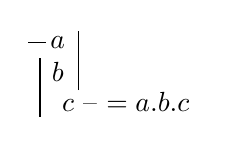
\begin{tikzpicture} [scale=.75]
%\draw[help lines, color=red!25] (-1,-1) grid (4,2);
\SetGraphUnit{1}    \GraphInit[vstyle=Empty]    
\node  (a) at (0,1) {$a$} ;  
\node  (b) at (0,.5) {$b$} ;  
\node  (c) at (1.15,0) {$c$ -- $= a.b.c$ } ;  
\draw (-.5,1) -- (-.2,1) ; 
\draw (-.3,-.25) -- (-.3,.75) ; 
\draw (.35,.2) -- (.35,1.2) ; 
\end{tikzpicture}} 

Si l'on met, dans cette fonction, « $f_5$ » en facteur à droite, la simplification obtenue \footnote{{\emph{N.B.} -- Le trait vertical d'un produel, quand il n'est pas en extrémité, est équivalent au symbole d'un produit (.). Ce qui permet d'écrire : 
\raisebox{-9mm} {\box1}
}}, 



\centerline{\begin{tikzpicture} [scale=.75]
%  \draw[help lines, color=red!25] (-1,-1) grid (7,5);
\SetGraphUnit{1}    \GraphInit[vstyle=Empty]    
% \node  (O) at (0,0) {$\times$} ;  
\node [VertexStyle] (a) at (1,3.5) {$f_1$} ;  
\node [VertexStyle] (b) at (1,.5) {$f_2$} ;  
\node [VertexStyle] (c) at (3.25,2) {$f_3$} ;   
\node [VertexStyle] (d) at (6,.5) {$f_4$} ;   
\node [VertexStyle] (e) at (6,3.5) {$f_5$} ;   
\draw [thick]  (-.5,2 ) -- (0, 2) -- (0,0.5) -- (b) -- (d)  -- (7,.5) -- (7,3.5) -- (e) -- (a)   ;   
\draw [thick]  (0, .5) -- (0,3.5) -- (a)  ;   
\draw [thick]  (2,.5) -- (2, 2) -- (c)  -- (4.5, 2) -- (4.5, 3.5)  ;   
\draw [very thick]  (a.south)  -- (5.25, 3)  to  [bend  left=90] ( 5.25, 1.5)  -- (3.75,1.5)   to  [bend  right=90] ( 3.75,1) ;  
\draw [very thick,->,>=latex]  ( 3.75,1) -- (6,1)  ;  
\end{tikzpicture}
} 

fait apparaître suivant le parcours indiqué par la flèche le produit $f_1 . f_2 . f_4$ qui n'était pas contenu initialement dans la fonction proposée. Cette simplification ne peut pas être effectué si  $f_1 . f_2 . f_4 \neq 0$. \\
Nous pouvons par contre effectuer une simplification par mise en facteur de droite à gauche, dans la fonction suivante : 




\setbox1=\hbox{ $ \begin{vmatrix}
x_1 . \overline{x_2} .  \overline{x_3} \\
\overline{x_1} . x_2 .  \overline{x_3} \\
\overline{x_1}  .  \overline{x_2} . x_3 \\       
\end{vmatrix} =$ }


\centerline{\begin{tikzpicture} [scale=.75]
% \draw[help lines, color=red!25] (-4,0) grid (7,5);
\SetGraphUnit{1}    \GraphInit[vstyle=Empty]    
\node [VertexStyle] (A) at (-1.75, 2) {\box1} ;  
% \node [red]  (O) at (0,0) {$\times$} ;  
\node [VertexStyle] (a) at (1.75,1) {$ \overline{x_1}$} ;  
\node [VertexStyle] (b) at (3,3) {$ x_1 . \overline{x_2}$} ;  
\node [VertexStyle] (c) at (4,1.5) {$x_2$} ;  
\node [VertexStyle] (d) at (4,0.5) {$ \overline{x_2}$} ;  
\node [VertexStyle] (e) at (5.75,0.5) {$ x_3$} ;  
\node [VertexStyle] (f) at (5.75,2.5) {$ \overline{x_3}$} ;  
\draw [thick] (A) -- (1,2) -- (1,1) -- (a)  ; 
\draw [thick] (1,2) -- (1,3) -- (b) ; %  -- (5,3) -- (5,.5) -- (d) -- (3,.5) -- (3, 1.5) -- (c)  ; 
\draw [thick]  (a) -- (3, 1) -- (3,.5) -- (d) -- (e) ;  
\draw [thick]  (3, 1)  -- (3,1.5) -- (c) -- (4.75, 1.5) -- (4.75,3) -- (b) ; 
\draw [thick]  (4.75, 2.5) --   (f) -- (7.75, 2.5)  ; 
\draw [thick]  (6.75, 2.5) --   (6.75, .5) -- (e)   ; 
\draw [very thick]  (2.25, 2.65)  -- (5, 2.65)   to  [bend  left=90] (4.85, 1.3) --  (3.75,1.3)   to  [bend  right=90] ( 3.75,1) ;  
\draw [very thick,->,>=latex]  ( 3.75,1) -- (6,1)  ;  
\end{tikzpicture}
} 



Le produit $x_1 .  \overline{x_2} . x_2 .  \overline{x_2} . x_3 $ indiqué par la flèche est identiquement nul puisqu'il contient en facteur deux variables complémentaires $x_2$ et  $\overline{x_2}$ . Il n'y a donc pas de modification introduite dans la fonction initiale et la simplification obtenue est valable. \\
Notons que dans certains cas, la solution particulière introduite est \emph{redondante} et permet d'améliorer la simplification. C'est le cas de la fonction suivante : 
 
\setbox1=\hbox{ $ \begin{vmatrix}
f_1 . f_4\\
f_1 . f_2 . f_3 \\
f_5 . f_2 \\
f_5 . f_3 . f_4\\ 
\end{vmatrix} = \dfrac{\quad}{\quad}$ }





\centerline{\begin{tikzpicture} [scale=.75]
% \draw[help lines, color=red!25] (-4,0) grid (13,5);
\SetGraphUnit{1}    \GraphInit[vstyle=Empty]    
\node [VertexStyle, fill opacity=0.2, text opacity=1] (A) at (-1.75, 2) {\box1} ;  
% \node [red]  (O) at (0,0) {$\times$} ;  
\node [VertexStyle] (c) at (3,3.5) {$f_4$} ;  
\node [VertexStyle] (d) at (3,2.5) {$f_3 . f_2$} ;  
\node [VertexStyle] (e) at (3,1.5) {$f_2$} ;  
\node [VertexStyle] (f) at (3,0.5) {$f_3 . f_4$} ;  
\node [VertexStyle] (g) at (1,1) {$f_5$} ;  
\node [VertexStyle] (h) at (1,3) {$f_1$} ;  
\draw [thick]   (0,2)  -- (0,1)  -- (g)  -- (1.75, 1) -- (1.75,.5) -- (f)   -- (4.5, .5) -- (4.5, 3.5) -- (c) -- (1.75, 3.5) -- (1.75, 2.5) -- (d)  -- (4.5, 2.5) ;  
\draw [thick]   (0,2) -- (0,3) -- (h) -- (1.75, 3) ; 
\draw [thick]   (1.75, 1) -- (1.75,1.5)  -- (e)  -- (4.5,1.5) -- (4.5, 2) -- (5,2) ; 
% 
\node [VertexStyle] (B) at (5.5,2) {$ = $} ;  
\node [VertexStyle] (i) at (7.25,3) {$f_1$} ;  
\node [VertexStyle] (j) at (7.25,1) {$f_5$} ;  
\node [VertexStyle] (k) at (9.25,2) {$f_3$} ; 
\node [VertexStyle] (l) at (11,2) {$f_2$} ; 
\node [VertexStyle] (m) at (11,1) {$f_3 . f_4$} ; 
\node [VertexStyle] (n) at (10,4) {$f_4$} ; 
\draw [thick]   (B) -- (6.25,2) -- (6.25, 3) -- (6.50, 3) -- (i) -- (8.25, 3) -- (8.25, 2) --   (k)  -- (l) -- (13, 2)  ; 
\draw [thick]   (6.25,3) -- (6.25, 1) -- (j) -- (10, 1) -- (10,2) -- (10, 1) -- (m) -- (12.5,1) -- (12.5,4) -- (n) -- (8.25, 4) -- (8.25, 2)  ; 
\draw [very thick] (7,1.25) -- (9,1.25) to  [bend  right=90] ( 9,1.7) -- (8.25,1.7)  to 
 [out=180, in=-90]  (7.9,2) -- (7.9,4)   to  [out=90, in=180]  (8.5, 4.5)  ;  
\draw [very thick,->,>=latex]  (8.5, 4.5)  -- (11, 4.5) ;
\draw [very thick,->,>=latex]  (7, .5) -- (12.5, .5)  ;
\end{tikzpicture}
} 

Les deux parcours indiqués par les flèches, correspondent au même produit « $ f_5 . f_3 . f_4 $ ». Le produit « $f3 . f_4$ » en facteur dual de « $ f_2 $ » peut, en conséquence, être supprimé sans que la fonction soit modifiée. Nous obtenons donc finalement : 


\centerline{\begin{tikzpicture} [scale=.75]
% \draw[help lines, color=red!25] (-4,0) grid (13,5);
\SetGraphUnit{1}    \GraphInit[vstyle=Empty]    
\node [VertexStyle, fill opacity=0.2, text opacity=1] (A) at (-1.75, 2) {\box1} ;  
%\node [red]  (O) at (0,0) {$\times$} ;  
\node [VertexStyle] (A) at (0,1) {$F = $} ;  
\node [VertexStyle] (a) at (2,2) {$(f_1)$} ;  
\node [VertexStyle] (b) at (6,0) {$(f_2)$} ;  
\node [VertexStyle] (c) at (4,1) {$(f_3)$} ;  
\node [VertexStyle] (d) at (6,2) {$(f_4)$} ;  
\node [VertexStyle] (e) at (2,0) {$(f_5)$} ;  
\draw [thick] (A) -- (1,1) -- (1,0) -- (e) -- (b) -- (7,0) -- (7, 2) -- (d) -- (a) -- (1,2) -- (1,1) ;
\draw [thick] (3,2) -- (3,1) -- (c) -- (5,1) -- (5,0) ; 
\end{tikzpicture}
} 

Le symbolisme choisi permet ainsi, par des mises en facteur simultanées de part et d'autre des expressions binaires, 'établir des liens étroits avec la topologie et d'aboutir à des expressions simples ayant l'aspect de schémas. 

Notons cependant que ces simplifications n'offrent d'intérêt que pour certains circuits utilisant une technologie où les éléments  sont à commande isolée (relais électromagnétiques, optoélectroniques ou transformateurs ). Ce n'est pas le cas des circuits électroniques utilisant des semi-conducteurs des types diode et transistor.

\end{itemize}

<h3>Décomposition des fonctions binaires par rapport aux variables</h3>

Il est intéressant, dans un but de simplification, d'étudier les différentes formes que peut revêtir une fonction binaire relativement à une variable indépendante. 

\subsection {Définitions.} Nous dirons, par définition, qu'une \emph{fonction est monoforme par rapport à la variable « $x$ » } si cette variable intervient dans la fonction sous une seule de ses formes binaire (directe ou complémentée).  

Nous dirons dans ce cas que « $x$ » \emph {est une variable monoforme} de la fonction.



 
 \centerline{ $f_1 .  \begin{vmatrix} x \\ f_2 \\
                               \end{vmatrix}$   et  $ 
                               \begin{vmatrix} \overline{x} . {\varphi}_1 \\  {\varphi}_2 \\
                               \end{vmatrix}$  }
 

  
\setlength {\parindent} {0mm}  
sont des \emph{fonctions monoformes} par rapport à la variable « $x$ » à condition que $f_1, f_2, . {\varphi}_1 \text{ et } {\varphi}_2 $ soient des fonctions indépendantes de  « $x$ ». 
\setlength {\parindent} {5mm}

Nous appellerons \emph{fonction biforme par rapport à la variable « $x$ »}, toute fonction binaire dans laquelle la variable « $x$ » intervient à la fois sous ses deux formes (directe et complémentée) et nous dirons que « $x$ » est une \emph{variable biforme} de la fonction.  




 \centerline{ $ {\varphi}_1 .   \left| \begin{array}{c|c} x  & \overline{x}\\ f_1 & f_2 \\
\end{array} \right| \quad \text{ et } \quad 
                               \begin{vmatrix} \overline{x} . f_1 \\
                               x . f_2 \\
                                  {\varphi}_1 \\
                               \end{vmatrix}$  }
 

 
\setlength {\parindent} {0mm}  
sont des \emph{fonctions biformes} par rapport à la variable « $x$ ».
\setlength {\parindent} {5mm} 


Nous dirons qu'une fonction binaire est \emph{un produit monoforme} de la variable « $x$ » lorsque « $x$ », ou « $\overline{x}$ », est \emph{un implicant direct de cette fonction}. 

\begin{itemize}
\item $ F = \overline{x} . A $ est un \emph{produit monoforme de la variable « $x$ »}. 

Un \emph{produel monoforme} de la variable « $x$ » admet cette varaible ou son complément comme \emph{implicant dual}.

\item $F' = \begin{vmatrix}
x \\ B \\
\end{vmatrix}$  est un \emph{produel monoforme de la variable « $x$ »}. 

Nous appellerons \emph{fonction carrée biforme}, une fonction biforme comprenant quatre termes groupée en carré suivant un produit de deux produels de deux facteurs duals, ou suivant un produel de deux produits de de deux facteurs direct 



\item   $  \begin{vmatrix}  {\varphi} + A  \\
                                 \overline{ \varphi} . B  \\
                               \end{vmatrix}
                                \quad \text{ et } \quad  
                                \left| \begin{array}{c|c} \varphi  & \overline{\varphi}\\ A_1 & B_2 \\
\end{array} \right| $ sont des \emph{fonctions carrées biformes en « $\varphi$ »}.
 
\end{itemize} 

\setbox1=\hbox{\footnote{L'algèbre de {\sc Boole} ne peut pas mettre en évidence d'une façon simple les proprétés fondamentales des fonctions carrées biformes qui ont une symétrie duale particulière et sont extrêmement utiles pour la simplification des circuits de commutation.}}


<h4>Propriétés des fonctions carrées biformes\protect\footnote{L'algèbre de {\sc Boole</h4> ne peut pas mettre en évidence d'une façon simple les proprétés fondamentales des fonctions carrées biformes qui ont une symétrie duale particulière et sont extrêmement utiles pour la simplification des circuits de commutation.} } Les \emph{fonctions  carrées biformes} ont un aspect dual qui laisse prévoir des propriétés particulièrement intéressantes.



\emph{Toute fonction peut s'écrire sous la forme d'une fonction carrée biforme}. 



\begin{itemize}
\item $f_1 . \begin{vmatrix}
                   x \\  f_2 
                 \end{vmatrix} 
                   =  \left| \begin{array}{c|c} 
                                  \overline{x} . x & x \\
                                  f_1 & f_2  \\
                             \end{array} \right|
                             = \left| \begin{array}{c|c|c}  
                                     \overline{x} &   x & x \\
                                       f_1 & f_1 & f_2  \\
                                      \end{array} \right| 
                                      = \left| \begin{array}{c|c} 
                                          \overline{x} . & x \\
                                          f_1 & f_1 . f_2  \\
                                     \end{array} \right| $ 


                                    
\item $ \begin{vmatrix}
\overline{x} . \varphi_1 \\
      \varphi_2       
\end{vmatrix}    = \begin{vmatrix}
                             \overline{x} . \varphi_1 \\
                             \begin{array}{c|ccc} 
                             \overline{x} &$\multirow{2}{*}{$\varphi_2$}$ \\
                             x   & \\
                             \end{array} 
                             \end{vmatrix}   = \begin{vmatrix}       
                                                               \begin{array}{c|c}
                                                             $\multirow{2}{*}{$\overline{x}$}$ & \varphi_1\\
                                                                                                           & \varphi_2\\                                              
                                                                \end{array} \\
                                                       x . \varphi_2 \\
                                                       \end{vmatrix}  
$



\item     $\varphi_1 .    \left| \begin{array}{c|c} 
                                x &     \overline{x}  \\
                                  f_1 & f_2  \\
                             \end{array} \right|    
                             =    \left| \begin{array}{c|c|c} 
                                            x   .   \overline{x} & x &   \overline{x}  \\
                                          \varphi_1 & f_1 & f_2  \\
                                         \end{array} \right|    
                                         =   \left| \begin{array}{c|c} 
                                            x    &   \overline{x}  \\
                                          \varphi_1 . f_1 & \varphi_1 . f_2  \\
                                         \end{array} \right|    
   $            
   
  


\item  $ \begin{vmatrix}
\overline{x} .f_1 \\
x . f_2 \\
\varphi_1 \\
\end{vmatrix} 
          = \begin{vmatrix}
                 \overline{x} . f_1 \\
                 x . f_2 \\
                  \begin{array}{c|c} 
                                            \overline{x}   & $\multirow{2}{*}{$\varphi_1$}$  \\
                                                     x  &  \\
                   \end{array}       
          \end{vmatrix}    
            = \begin{vmatrix}
            \begin{array}{c|c} 
               $\multirow{2}{*}{$\overline{x}$}$ & f_1 \\
                      & \varphi_1 \\ 
            \end{array} \\
                 & \\
            \begin{array}{c|c} 
            $\multirow{2}{*}{$x$}$ & f_2 \\
                       & \varphi_1
            \end{array} 
            \end{vmatrix}
$

Si une \emph{fonction carrée biforme} se présente sou sla forme d'un produit de produels ,   



\centerline{
$ P =   \left| \begin{array}{c|c} 
                                            \varphi    &   \overline{\varphi}  \\
                                                 A        &              B   \\
                                         \end{array} \right| 
$}



nous pouvons l'écrire  sous la forme de produel de produite en effectuant les produits élémentaires : 



\centerline {$
P =  
\begin{vmatrix}
                \varphi . B \\
                A . \overline{\varphi} \\
                A . B \\
\end{vmatrix}
                 = \begin{vmatrix}
                     \varphi . B \\
                     A   . \overline{\varphi}  \\      
                     \begin{array}{c|c} 
            $\multirow{2}{*}{$A . B $}$ & \varphi \\
                                      & \overline{\varphi}
                      \end{array}  \\ 
                  \end{vmatrix}
                       = \begin{vmatrix}
                             \begin{array}{c|c} 
            $\multirow{2}{*}{$\varphi $}$ & B  \\
                                      &A . B \\
                      \end{array}  \\
                       & \\
                              \begin{array}{c|c} 
            $\multirow{2}{*}{$\overline {\varphi}$}$ &  A  \\
                                      &A . B \\
                              \end{array}  \\
                       \end{vmatrix}
$}



\centerline{ $ \begin{vmatrix}
B \\ A.B \\
\end{vmatrix} = B$,  $ \qquad \begin{vmatrix}
A \\ A.B \\
\end{vmatrix} = A$}

d'ou : 



\centerline{
 $  \begin{vmatrix}  {\varphi} . A  \\
                                 \overline{ \varphi} . B  \\
                               \end{vmatrix}
                                \quad \text{ et } \quad  
                                \left| \begin{array}{c|c} \varphi  & \overline{\varphi}\\ A_1 & B_2 \\
\end{array} \right| $
}



Nous avons ainsi établi le théorème suivant ; théorème fondamental et très imporant qui va permettre la recherche systématique des implicants directs et duals d'une fonction, par la méthodes des consensus.

<h4>Théorème.</h4>  \emph{Une fonction carrée biforme n'est pas modifiée par la suppression ou le tracé d'un trait vertical médian, à condition de disposer les facteurs complémentaires suivant une diagonale du carré correspondant à son expression symbolique.}



\centerline{
 $  \begin{vmatrix}  {\varphi} . B  \\
                                 A . \overline{ \varphi}   \\
       \end{vmatrix}
                     \quad \equiv \quad 
                                \left| \begin{array}{c|c} 
                                     \varphi  & B \\
                                      A & \overline{\varphi} \\
                                \end{array} \right| $
}



Les facteurs « $A$ » et « $B$ » sont appelés simplement \emph{facteurs diagonaux} de la fonction carrée biforme. 

\emph{Ce théorème nous permet de passer ainsi facilement d'un produel à un produit et vice-versa, sans introduire de terme redondant}. Ce qui justifie l'attention particulière consacrée à l'étude des fonctions carrées biformes. 

\end{itemize}

<h3>Simplificationpar la méthode des « consensus »\protect \footnote{Rappelons pour mémoire qu'une théorie complète des consensus, dans le formalisme de l'algèbre de {\sc Boole</h3>, a été développée par Monsieur Tison}}

Étant donnée une fonction carrée biforme, on appelle « \emph{consensus} » de cette fonction, le produit des termes diagonaux non complémentaires, « \emph{consensus dual} » le produel des termes diagonaux non complémentaires. 



La fonction carrée biforme 



  \centerline{$
   F =      \left| \begin{array}{c|c} 
                                     \varphi  & f_1 \\
                                      f_2 & \overline{\varphi} \\
                                \end{array} \right| 
                                    \quad = \quad 
                  \begin{vmatrix}  {\varphi} . f_1  \\
                                 \overline{ \varphi} . f_2   \\
               \end{vmatrix}
$}

admet comme « consensus » le produit $f_1 . f_2$ et pour « consensus dual » le produel  $\begin{vmatrix} f_1 \\f_2 \\ \end{vmatrix}$. \\ 
En procédent par produits effectués, nous pouvons écrire : 




\centerline{ $ F = \begin{vmatrix}
\varphi . f_1 \\ f_2 \overline{\varphi}
\end{vmatrix} 
       = \begin{array}{|c|c|c|} 
           \varphi & f_1 & f_1 \\
            f_2 & \overline{\varphi} & f_2 \\
           \end{array} 
             = \begin{vmatrix}
               \varphi . f_1 \\
               f_2 .   \overline{\varphi}  \\
               f_2 . f_1 \\           
             \end{vmatrix}
$.}





Le consensus $f_1 . f_2$ est donc un implicant dual de « $F$ » et le consensus dual $\begin{vmatrix} f_1 \\ f_2 \\ \end{vmatrix} $ est un implicant de   « $F$ ». Nous en déduisons les théorèmes suivants. 

<h4>Théorèmes.</h4> \begin{enumerate}
\item Si parmi les facteurs d'un produit, il existe une fonction carrée biforme et un terme contenant un facteur dual, le consensus dual de cette fonction, ce dernier terme est redondant et peut être supprimé. 

\item Si parmi les facteurs  duals d'un produel, il existe une fonction carrée biforme et un terme contenant un facteur dual, le consensus dual de cette fonction, ce dernier terme est redondant et peut être supprimé. 

\end{enumerate} 

Nous pouvons écrire en effet : 




\begin{spreadlines}{12pt}
 \begin{alignat*}{2} \begin{array}{|c} 
                         \varphi . f_1 \\ f_2 . \overline{\varphi}
                    \end{array}
                     \begin{vmatrix}
                        k\\  f_1 \\  f_2 \\
                    \end{vmatrix}. f_3\ldots f_n 
                   &=   \begin{array}{|c} 
                            \varphi . f_1 \\
                            f_2 . \overline{\varphi}
                        \end{array}
                        \begin{array}{|c|c|} 
                            0 & k  \\
                            f_1 & f_2 \\
                            f_2 & f_2 \\
                        \end{array} . f_3\ldots f_n  \\
                   &= \begin{array}{|c} 
                         \varphi . f_1 \\ f_2 . \overline{\varphi}
                    \end{array}
                     \begin{vmatrix}
                     f_1 \\  f_2 \\
                    \end{vmatrix}. f_3\ldots f_n  \\
                         &= \begin{array}{|c|} 
                         \varphi . f_1 \\ f_2 . \overline{\varphi}
                    \end{array}
                   . f_3\ldots f_n  \\
\end{alignat*}
\end{spreadlines}

De même : 

\[ 
      \begin{vmatrix}
          \varphi . f_1\\ f_2 . \overline{\varphi} \\ k . f_1 . f_2 \\ f_3 \\ \vdots \\ f_n \\
      \end{vmatrix} 
       =   \begin{vmatrix}
                  \varphi . f_1\\ f_2 . \overline{\varphi} \\ 1 . f_1 . f_2 \\  k . f_1 . f_2 \\ f_3 \\ \vdots \\ f_n \\
             \end{vmatrix}
             =   \begin{vmatrix}
                                       \varphi . f_1\\ f_2 . \overline{\varphi} \\  f_1 . f_2 \\  f_3 \\ \vdots \\ f_n \\
                  \end{vmatrix} 
                  =  \begin{vmatrix}
                                       \varphi . f_1\\ f_2 . \overline{\varphi}  \\  f_3 \\ \vdots \\ f_n \\
                    \end{vmatrix} 
\]

<h4>Règles générales des « consensus ».</h4> Donnons-nous la fonction carrée biforme : 

\[
   F =      \left| \begin{array}{c|c} 
                      \varphi  & f_2 \\
                      f_1 & \overline{\varphi} \\
                   \end{array} \right| 
                                   =
                  \begin{vmatrix}  {\varphi} . f_2  \\
                                f_1 .  \overline{ \varphi}   \\
                  \end{vmatrix}
\]


 \begin{itemize}
 \item Le \textsf{consensus} « $f_1 . f_2$ » mis sous la forme d'un produel de produits, traduit, lorsque l'un des produits apparaît en facteur dans un terme facteur dual de « $F$ », une condition suffisante pour affirmer que ce terme est redondant et peut être supprimé.
 
  \item Le \textsf{consensus dual} $ \begin{vmatrix} f_1 \\ f_2 \\ \end{vmatrix}$ mis sous la forme d'un produit de produel, traduit, lorsque l'un des produits apparaît en facteur dual dans un terme facteur de « $F$ », une condition suffisante pour affirmer que ce terme est redondant et peut être supprimé.
 
 \end{itemize}
 


 Supposons que le consensus de la fonction carrée biforme « $F$ » soit mis sous la forme d'un produel de « $q$ » produits : 
 
 \[ f_1 . f_2 = \begin{vmatrix} p_1 \\ p_2 \\ \vdots \\ p_k  \\ \vdots \\ p_q \end{vmatrix}\text{,} \]
 
 et que le consensus dual soit mis sous  la forme d'un produit de « $r$» produels : 
 
\[ \begin{array}{|c|} f_1 \\ f_2 \\ \end{array} = \pi_1 . \pi_2\ldots \pi_j\ldots \pi_r  \]


 
 Si la fonction « $F$ » est ub dacteur dual d'un terme de la forme « $Ap_k$ », ce terme est redondant.
 
 Nous pouvons écrire en effet dans ce cas : 
 
 \[ \begin{vmatrix}
 F\\ A.p_k
 \end{vmatrix} = \begin{vmatrix} F \\  f_1 . f_2 \\ A . p_k \\\end{vmatrix} 
               = \begin{vmatrix} F \\ p_1 \\ p_2 \\ \vdots \\ p_k \\ \vdots \\ p_q \\A.p_k\\ \end{vmatrix}
 \]
 
 « $p_k$ » implicant de « $A . p_k$ », est un facteur dual et nous savons que : 
 
\[ 
\begin{array}{|c|}
     p_k \\ 
     A . p_k \\ 
\end{array} 
     = p_k 
\] 
 
 
 d'où : 
 
\[ \begin{array}{|c|} F  \\ f_1 . f_2  \\ A . p_k \\ \end{array} 
   = \begin{array}{|c|} F \\ f_1 . f_2  \\ \end{array}  = F \] 
  
  Si la fonction « $F$ » est en facteur d'un terme de la forme $\begin{array}{|c|}
    B \\ 
     \pi_j \\ 
\end{array}$, nous pouvons écrire : 
  
\[ F . \begin{array}{|c|} B \\ \pi_j \\ \end{array} = F . \begin{array}{|c|c|} f_1 & G \\ f_2 & \pi_j \\ \end{array}
    = F . \pi_1 . \pi_2\ldots \pi_j . \begin{array}{|c|} B \\ \pi_j \end{array} . \pi_{j+1}\ldots \pi_r   \]
    
$\pi_j$ est un implicant dual du produel      $\begin{array}{|c|} B \\ \pi_j \end{array}$ \\
donc, 

\[ F . \begin{array}{|c|c|} f_1 & B \\ f_2 & \pi_j \\ \end{array} 
        = F . \begin{array}{|c|} f_1 \\ f_2 \end{array} = F \text{.}    
\] 

<h4>Exemple de simplification par consensus.</h4> Conisdérons la fonction 

\[ F_1 = \begin{array}{|l|} B . C . F \\
                            D . \overline{C} . F \\
                            D . B . E \\
                            A . \overline{C} \\
                            D . \overline{A}\\
                            A . B \end{array} \begin{array}{c|} D \\ B \\ \overline{C} \\ \overline{F}\end{array} 
\]

Il existe, dans le premier facteur de  « $F_1$ » deux variables biformes « $C$ » et « $A$ » et nous pouvons faire apparaître successivement les deux fonctions carrées biformes : 

\[  \begin{array}{|c|} C . B . F \\
           \begin{array}{c|c} D . F & $\multirow{2}{*}{$\overline{C}$}$\\
                                  A & \\            \end{array} 
\end{array}                             
                    \quad   \text { et } \quad 
              \begin{array}{|c|c|} 
             $\multirow{2}{*}{$\overline{A}$}$ & \overline{C} \\
                          & B \\
\multicolumnn{2}{|c|}{D . \overline{A} }  \\          
              \end{array} 
\] 

qui admettent respectivement pour \emph{consensus} : 

\[ \begin{array}{|c|} B . D . F \\ A . B . F \end{array} \text{,} \quad \begin{array}{|c|} D \overline{C} \\ D . B \\ \end{array} \text{,} \]  


et admettent pour \emph{consensus dual} : 

\[ \begin{array}{|c|} 
	A \\ D \\ B \\ 
\end{array} 
      \begin{array}{c|} 
           A \\ F \\ 
      \end{array}   
            \quad \text{ et } \quad 
                  \begin{array}{|c|} D \\ B \\ \overline{C} \end{array} \]

Nous voyons, par le consensus de la fonction carré biforme en « $A$ », consensus égal à $ \begin{array}{|c|} D . B \\ D \overline{C} \end{array}$, que les termes $ D . \overline{C} . F$ et $ D . B  . E $ peuvent être supprimés. Nous pouvons donc écrire : 

 
\[ 
F_1 = \begin{array}{|c|c|c|} 
            $\multirow{2}{*}{$A$}$ & \overline{C} & D \\
                                   &   B          & B \\
\multicolumnn{2}{|c|}{D . \overline{A}} & \overline{C} \\
\multicolumnn{2}{|c|}{B . C . F }   & \overline{F} \\  
             \end{array} 
             = 
           \begin{array}{|c|c|c|} 
                     A & \overline{C} & D \\                    
                      &              & B  \\
                    $\multirow{3}{*}{$D$}$    &       B        &   \\
                     	  &  & \overline{C}  \\
                     	  & \overline{A} & \overline{F}  \\
\multicolumnn{3}{|c|}{B . C . F }  \\	  
          	\end{array}                          
\]


Le produel $ \begin{array}{|c|} D \\ B \\ \overline{C} \\ \overline{F} \end{array} $  contient le consensus dual $\begin{array}{|c|} D \\ B \\ \overline{C} \\ \end{array} $


d'où, 

\[ 
F_1 = \begin{array}{|c|} 
         \begin{array}{c} A \\ D \\\end{array} \begin{array}{|c} \overline{C} \\ B \\ \overline{A} \\ \end{array} \\
         B . C . F  
 \end{array} = \begin{array}{|l|} A . \overline{C} \\ A . B \\ D . \overline{A}  \\ B . C . F \end{array} 
\] 

Nous pouvons encore écrire : 

\[
F_1 = \begin{array}{|c|c|} A & \overline{A}\\ D & B \\ B . C . F & \overline{C}\\ \end{array} 
    = \begin{array}{|c|c|c|c|} A & A & A & \overline{A} \\ D & D & D & B \\ B & C & F & \overline{C}\\\end{array}  
\] 



La recherche des consensus conduit souvent à la simplification optimale des fonctions binaires. Elle complète utilement les méthodes se simplification par mise en facteur, transposition et adjacences. 

Ces quatre méthodes combinées permettent, en général, lorsqu'elles sont utilisées judicieusement, d'obtenir les formes minimales. 

<h3>Simplifications par adjacences</h3>

Les simplifications par adjacences sont les premières qu iont été utilisées en algèbre de « \textsc{Boole} ». Elles étaient, alors, les plus faciles à mettre en œuvre et ont donné naissance à différentes méthodes comme celle établie par « \textsc{Quine} et \textsc{Mc Cluskey} » ou celle des diagrammes de « \textsc{Venn} » et de « \textsc{Veitch} » que nous citons simplement pour mémoire. 

Nous développerons, par contre, la méthode des diagramme de « \textsc{Karnaugh} » parce que ces diagrammes sont assimilables aux tracés des tables de vérité particulières dans lesquelles les adjacences sont topologiquement groupées ou bien se correspondent géométriquement par symétrie. 

Le diagramme de \textsc{Karnaugh} se présente sous la forme d'un carré ou d'un rectangle selon la parité du nombre de variables. L'ensemble des variables est généralement partagé en deux sous-ensembles contenant, à une unité près, le même nombre de variables. 

Au nombre de combinaisons de valeurs de ces deux sous-ensembles, on fait correspondre, respectivement, le nombre des cases de chacun des côtés du rectangle ou du carré. Il suffit ensuite de ranger les combinaisons de valeurs des varaibles dans un ordre respectant les adjacences par groupements ou symétries comme le précisent les exemples suivants : 




\textbf{Cas de deux variables.} 

\centerline{ \begin{tabular}{c|c|c|}
\multicolumnn{1}{c}{\diagbox[width=10mm]{A}{B}}  
         & \m\multicolumnn{1}{c}{0} 
               & \m\multicolumnn{1}{c}{1} \\
      \cline{2-3}
\multicolumnn{1}{c|}{0} & 0 & 1 \\
           \cline{2-3}
\multicolumnn{1}{c|}{1} & 2 & 3 \\
           \cline{2-3}
\end{tabular}}

\textbf{Cas de trois variables.} 

\centerline{ \begin{tabular}{c|c|c|c|c|}
\multicolumnn{1}{c}{\diagbox[width=15mm]{A}{BC}}  
         & \m\multicolumnn{1}{c}{00} 
               & \m\multicolumnn{01}{c}{01} 
                    & \m\multicolumnn{1}{c}{11} 
                        & \m\multicolumnn{01}{c}{10} \\
      \cline{2-5}
\multicolumnn{1}{c|}{0} & 0 & 1 & 3 & 2\\
           \cline{2-5}
\multicolumnn{1}{c|}{1} & 4 & 5 & 7 & 6 \\
           \cline{2-5}
\end{tabular}}

\textbf{Cas de quatre variables.} 

\centerline{ \begin{tabular}{c|c|c|c|c|}
\multicolumnn{1}{c}{\diagbox[width=15mm]{AB}{CD}}  
         & \m\multicolumnn{1}{c}{00} 
               & \m\multicolumnn{01}{c}{01} 
                    & \m\multicolumnn{1}{c}{11} 
                        & \m\multicolumnn{01}{c}{10} \\
      \cline{2-5}
\multicolumnn{1}{c|}{00} & 0 & 1 & 3 & 2\\
           \cline{2-5}
\multicolumnn{1}{c|}{01} & 4 & 5 & 7 & 6 \\
           \cline{2-5}
\multicolumnn{1}{c|}{11} & 12 & 13 & 15 & 14 \\
           \cline{2-5}
\multicolumnn{1}{c|}{10} & 8 & 9 & 11 & 10 \\
           \cline{2-5}     
\end{tabular}}

\textbf{Cas de cinq variables.} 


\sbox0{ \begin{tabular}{c|c|c|c|c||c|c|c|c|c|}
% \m\multicolumnn{9}{c}{\emph{\hspace*{2.5cm} axe de symétrie}} \\
\multicolumnn{1}{c}{\diagbox[width=20mm]{AB}{CDE}}  
         & \m\multicolumnn{1}{c}{000} 
               & \m\multicolumnn{01}{c}{001} 
                    & \m\multicolumnn{1}{c}{011} 
                        & \m\multicolumnn{01}{c}{010} 
                            & \m\multicolumnn{1}{c}{110} 
                              & \m\multicolumnn{01}{c}{111} 
                                 & \m\multicolumnn{1}{c}{101} 
                                    & \m\multicolumnn{01}{c}{100} \\
      \cline{2-9}
\multicolumnn{1}{c|}{00} & 0 & 1 & 3 & 2 & 6 & 7 & 5 & 4 \\
           \cline{2-9}
\multicolumnn{1}{c|}{01} & 8 & 9 & 11 & 10 &  14 & 15 & 13 & 12 \\
           \cline{2-9}
\multicolumnn{1}{c|}{11} & 24  & 25 & 27 & 26 &  30 & 31 & 29 & 28  \\
           \cline{2-9}
\multicolumnn{1}{c|}{10} & 16 & 17 & 19 & 18 &  22 & 23 & 21 & 20  \\
           \cline{2-9}     
\end{tabular}}

\centerline{
\usebox0 
\kern -27mm 
\llap
{
\raisebox{11mm}
{
\fboxsep0pt
\parbox{30mm} {
\begin{center}
                     axe de symétrie\\

                            $\downarrow$
                       \end{center}
}
}}
}



Il est intéressant, comme cela est fait sur les exemples traités, de repérer chaque case par l'équivalent décimal du nombre binaire associé à la combinaison de valeurs qui lui correspond.


Pour utiliser le diagramme de  « \textsc{Karnaugh} », on porte dans chacune des cases du carré ou du rectangle, la valeur que prend la fonction binaire envisagée pour la combinaison de valeurs des variables qui correspondent justement à cette case. Puis on constitue une table de vérité réduite, soit par rapport aux « $0$ » soit par rapport aux « $1$ » de la fonction selon ce qui paraît le plus simple, en tenant compte des adjacences possibles qui sont localisées avec facilité grâce à la distribution topologique particulière du diagramme. Il suffit ensuite d'établir la fonction à partir de la table de vérité réduite. Avec un peu d'habitude, on peut tirer la fonction directement du diagramme sous forme de produits ou de produels.

La méthode du diagramme de « \textsc{Karnaugh} » est intéressante et permet des simplifications rapides, mais présente l'inconvénient de n'utiliser que les adjacences comme mode de recherche des implicants. Le chaix des groupements et des symétries reste arbitraire et la méthode des mises en facteur et celle des consensus la complète utilement. 


<h4>Exemples.</h4> Les variables étant rangées dans l'ordre $A, B, C, D,$ écrire à l'aide du diagramme de  « \textsc{Karnaugh} »  la fonction binaire simplifiée égale à zéro pour les combinaisons $ 3\;(0011)$, $7\; (0111)$, $8\, (1000)$, $9\; (1001)$, $14\, (1110)$  et $15\, (1111)$ des valeurs des variables. 

On trace le diagramme de \textsc{Karnaugh} pour les quatre variables $A$, $B$, $C$ et $D$. On inscrit « $0$ » dans les cases correspondant à 3, 7, 8, 9, 14 et 15 et  « $1$ » dans les autres cases. 


% $\multirow{2}{*}{$\overline{x}$}$ 

\newsavebox{\speciesone}
\sbox{\speciesone}{
\begin{tabular}{c|cc|cc|cc|cc|}
\multicolumnn{1}{c}{\diagbox[width=15mm]{AB}{CD}}  
         & \m\multicolumnn{2}{c}{00} 
               & \m\multicolumnn{2}{c}{01} 
                    & \m\multicolumnn{2}{c}{11} 
                        & \m\multicolumnn{2}{c}{10} \\
      \cline{2-9}
  
ultirow{2}{*}{00}   & 1 & & 1 & & 0 & & 1 & \\
                               &  & 0 & & 1 & & 3 & & 2 \\                                  
           \cline{2-9}
ultirow{2}{*}{01}  & 1 & & 1 & & 0 & & 1 & \\
                     & & 4 && 5 && 7 && 6 \\
                      \cline{2-9}          
      
ultirow{2}{*}{11}  & 1 & & 1 && 0 & & 0 & \\
                     & & 12 && 13 & & 15&  & 14 \\
           \cline{2-9}          
ultirow{2}{*}{10}  & 0 && 0 && 1 && 1 & \\
                     & & 8 && 9 && 11 && 10 \\
           \cline{2-9}               
\end{tabular}}


\centerline{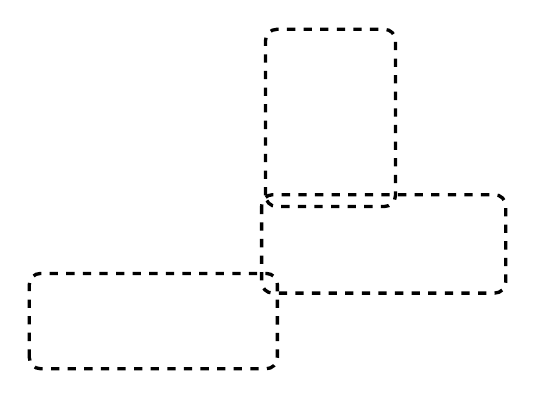
\begin{tikzpicture} [rounded corners] 
% \draw[help lines, color=red!20] (-4,-3) grid (4,3);
atrix [matrix of nodes] {
\node (species1)% [shape=rectangle,draw]
 {\usebox{\speciesone}};\\
};
\draw [very thick,dashed]   (.75,-.6) rectangle (2.4,1.65)  ; 
\draw [very thick,dashed]   (.7,-.45) rectangle (3.8,-1.7)  ; 
\draw [very thick, dashed]   (-2.25,-2.66) rectangle (.9,-1.45)  ; 
\end{tikzpicture}}



En groupant les cases adjacentes 3-7, 8)9, 14-15 on obtient la table de vérité réduite suivante : 



\centerline{
\begin{tabular}{c|c|c|c|c||c|}
\cline{2-6}
\emph{Combinaisons} & \multirow{2}{*}{A} &  \multirow{2}{*}{B}  &  \multirow{2}{*}{C}  &  \multirow{2}{*}{D}  &  \multirow{2}{*}{F} \\
\emph{groupées} & & & & & \\
\cline{2-6}
3 - 7 & 0 & $\phi$ & 1 & 1 & 0 \\
8 - 9 & 1 & 0 & 0 & $\phi$  & 0 \\
14 - 15   & 1 & 1 & 1 & $\phi$ & 0 \\
\cline{2-6} 
\end{tabular}
}



Ce qui permet d'écrire : 


\centerline{$ F = 
\begin{array}{|c|c|c|} 
	 A & \overline{A} &   \overline{A} \\
	\overline{C} & B & B \\
	\overline{D} & C & \overline{C} \\
\end{array}
$}



Mais on peut aussi bien grouper les cases adjacentes 

\smallskip 

\centerline {$0-1-4-5, \qquad 0-2-4-6, \qquad 4-5-12-13, \qquad 10-11$  } 

et l'on obtient la table de vérité réduite relative aux « $1$ » de la fonction binaire. 



\centerline{
\begin{tabular}{c|c|c|c|c||c|}
\cline{2-6}
\emph{Combinaisons} & \multirow{2}{*}{A} &  \multirow{2}{*}{B}  &  \multirow{2}{*}{C}  &  \multirow{2}{*}{D}  &  \multirow{2}{*}{F} \\
\emph{groupées :} & & & & & \\
\cline{2-6}
$0 - 1 -4 -5 $  & 0 & $\phi$ & 0 & $\phi$     & 1 \\
$0-2-4-6$       & 0 & $\phi$  &  $\phi$ & 0   & 1 \\
$4-5-12-13 $    & $\phi$  & 1 & 0 & $\phi$    & 1 \\
$10-11$         & 1 & 0 & 1 & $\phi$          & 1 \\   
\cline{2-6} 
\end{tabular}
}


Ce qui donne :




\centerline{$ F = 
\begin{array}{|l|} 
	 \overline{A} .  \overline{C} \\
	  \overline{A} .  \overline{D} \\
	  B .  \overline{C} \\
	  A .  \overline{B} . C \\ 
\end{array}
$}



En utilisant les propriétés des fonctions carrées biformes, on peut écrire successivement : 


\centerline{$ F = 
\begin{array}{|l|}  
	 \overline{A} .  \overline{C} \\
	 \overline{A} .  \overline{D} \\
	 \overline{A} . B  \overline{C} \\
	 A . B .  \overline{C} \\
	 A . B . C \\    
\end{array}
    = \begin{array}{|c|c|} 
           $\multirow{3}{*}{$\overline{A}$}$ & \overline{C} \\
                              & \overline{D} \\
                              & B . \overline{C} \\
\multicolumnn{2}{|c|}{} \\
          B .\overline{C} &    $\multirow{2}{*}{$A$}$ \\
          C . \overline{B} &   \\                    
      \end{array} 
         = \begin{array}{|c|c|c|} 
\multicolumnn{2}{|c|}{\overline{A}} & A \\
          B & \overline{C} & \overline{C} \\
          C & \overline{B} & \overline{D}
           \end{array} 
            = \begin{array}{|c|c|c|} 
            		\overline{A} & \overline{A} & A \\
            		B & \overline{B} & \overline{C} \\
            		C & \overline{C} & \overline{D} \\
               \end{array} 
$}



Le diagramme de \textsc{Karnaugh} se révèle vraiment utile dans le cas où les fonctions binaires sont incomplètement définies et présentesnt un certain nombre de combinaisons de variables disponibles qui ne sont jamais réalisées et pour lesquelles nous pouvons attribuer à la fonction aussi bien la valeur « $1$ » sue la valeur  « $0$ » selon les simplifications possibles. 

Donnons-nous, par exemple, une fonction de cinq variables $x_5$,   $x_4$, $x_3$, $x_2$, $x_1$ rangées dans l'ordre inverse des indices pour pouvoir leur faire correspondre les puissances de « $2$ » des nombres binaires associés. 


Il s'agit d'écrire la fonction  « $F$ » égale à l'unité pour les combinaisons $1-3-7-8-10-12-17-20$;

\begin{itemize}
\item Les combinaisons disponibles sont les suivantes : 

\[ 0-5-6-9-11-14-16-18-21-22\text{.} \]

La fonction est égale à zéro pour les combinaisons qui n'ont pas été considérées, c'est-à-dire :

\[ 2-4-13-15-19-23-24-25-26-27-28-29-30-31\text{.} \]

Les données permettent de tracer le diagramme de \textsc{Karnaugh} suivant :



\begin{tabular}{c|cc|cc|cc|cc||cc|cc|cc|cc|}
\multicolumnn{1}{c}{\diagbox[width=22mm]{$x_5x_4$}{$x_3x_2x_1$}}  
         & \m\multicolumnn{2}{c}{000} 
               & \m\multicolumnn{2}{c}{001} 
                    & \m\multicolumnn{2}{c}{011} 
                        & \m\multicolumnn{2}{c}{010} 
                                     & \m\multicolumnn{2}{c}{110} 
            							   & \m\multicolumnn{2}{c}{111} 
                   							 & \m\multicolumnn{2}{c}{101} 
                      							  & \m\multicolumnn{2}{c}{100} \\
      \cline{2-17}
  
ultirow{2}{*}{00}   & $\phi$ & & 1 & & 1 & & 0 & &  $\phi$ && 1 && $\phi$ && 0 & \\
                               &  & 0 & & 1 & & 3 & & 2  & & 6 && 7 && 5 && 4\\                               
           \cline{2-17}
ultirow{2}{*}{01}  & 1 & & $\phi$  & & $\phi$  & & 1 & &$ \phi$ && 0 && 0 && 1 & \\
                     & & 8 && 9 && 11 && 10 && 14 && 15 && 13 && 12 \\
           \cline{2-17}               
ultirow{2}{*}{11}  & 0 & & 0 && 0 & & 0 && 0 && 0 && 0 && 0 &  \\
                     & & 24 && 25 & & 27 &  & 26 && 30 && 31 && 29 && 28  \\
           \cline{2-17}          
ultirow{2}{*}{10}  & $\phi$  && 1 && 0 &&  $\phi$  &&  $\phi$ && 0 &&  $\phi$  && 1&  \\
                     & & 16 && 17 && 19 && 18 && 22 && 23 && 21 && 20  \\
           \cline{2-17}               
\end{tabular}



Nous pouvons tirer du diagramme, la table de vérité réduite relative aux valeurs « $1$ » de la fonction « $F$ » en utilisant au mieux les combinaisons disponibles repérées par le symbole « $\phi$ ».




\centerline{
\begin{tabular}{c|c|c|c|c|c||c|}
\cline{2-7}
\emph{Combinaisons} & \multirow{2}{*}{$x_5$} &  \multirow{2}{*}{$x_4$}  &  \multirow{2}{*}{$x_3$}  &  \multirow{2}{*}{$x_2$}  &  \multirow{2}{*}{$x_1$}  &  \multirow{2}{*}{$F$} \\
\emph{groupées :} & & & & & & \\
\cline{2-7}
$ 1-3-5-7$  & 0 & 0 & $\phi$ & $\phi$    & 1 & 1 \\
$8-10-12-14$       & 0 & 1 & $\phi$  &  $\phi$ & 0   & 1 \\
$16-17-20-21$   & 1 & 0  & $\phi$  &  0 & $\phi$    & 1 \\  
\cline{2-7} 
\end{tabular}
}



d'où : 


\centerline{$ F = 
\begin{array}{|c|} 
    \overline{x_5} . \overline{x_4} . x_1 \\
    \overline{x_5} . x_4 . \overline{x_1} \\
    x_5 . \overline{x_4} \overline{x_2} \\
\end{array}
    = \begin{array}{|c|c|}
            $\multirow{2}{*}{$\overline{x_5}$}$   & \overline{x_4} . x_1  \\
                                            & \overline{x_1} . x_4 \\
 %             \m\multicolumnn{2}{|c|}{} \\
\multicolumnn{2}{|c|}{\overline{x_4}.\overline{x_2}.x_5 }\\
       \end{array} 
$}



\centerline{$ F= 
\begin{array}{|c|c|} 
	x_1 & \overline{x_1} \\  
	x_4 & \overline{x_4} \\
	x_5 & x _5 \\   
 \end{array} \begin{array}{c|c|} 
                \overline{x_2} & \overline{x_4} \\
                \overline{x_5} & \overline{x_5} \\
             \end{array} 
             = \begin{array}{|c|} 
                 x_1 \\
                 x_4 \\
                 x_5 \\
                \end{array} 
                    \begin{array}{c|c|c|} 
                       \overline{x_4} & \overline{x_4} & \overline{x_2} \\
                       \overline{x_1} & \overline{x_5} & \overline{x_5}   \\
                    \end{array}  
$}



Nous pouvons également dresser une table de vérité réduite relative aux zéros de la fonction  $F$ » en utilisant les combinaisons disponibles 




\centerline{
\begin{tabular}{c|c|c|c|c|c||c|}
\cline{2-7}
\emph{Combinaisons groupées :} & {$x_5$} &   {$x_4$}  &   {$x_3$}  &   {$x_2$}  &   {$x_1$}  &   {$F$} \\
\cline{2-7}
$0-2-4-6$  & 0 & 0 & $\phi$ & $\phi$    & 0& 0 \\
$9-11-13-15-25-27-29-31$    &  $\phi$   & 1 &  $\phi$  & $\phi$  &  1    & 0 \\
$24-25-26-27-28-29-30-31$  & 1 & 1  & $\phi$  &   $\phi$  & $\phi$    & 0 \\  
$18-19-22-23-26-27-30-31$ & 1 & $\phi$   & $\phi$  & 1 & $\phi$    & 0 \\  
\cline{2-7} 
\end{tabular}
}



d'où 


\centerline{$ F = 
\begin{array}{|c|}  x_1 \\ x_4 \\ x_5     \end{array}
      \begin{array}{c|c|c|c|} 
           \overline{x_1} & \overline{x_4} & \overline{x_2} \\
           \overline{x_4} &\overline{x_5} &\overline{x_5}  \\    
      \end{array} 
         = \begin{array}{|c|c|} 
         	x_1 & \overline{x_1} . \overline{x_5} \\
         	x_4 & \overline{x_2} . \overline{x_4} \\
         	x_5 & \overline{x_4} . \overline{x_5} \\ 	
         \end{array} 
$}



Nous pouvons également écrire « $F$ » sous la forme :


\centerline{$ F = 
\begin{array}{|c|} \overline{x_5} . \overline{x_1} . x_4 \\
                   \overline{x_5} . x_1 . \overline{x_4} \\
                   x_5 . \overline{x_2} . \overline{x_4} \\  
                   \end{array} 
                     = \begin{array}{|c|c|c|}
                        $\multirow{2}{*}{$\overline{x_5}$}$    & \m\multicolumnn{2}{|c|}{\overline{x_1} . x_4} \\
                                                               & x_1 & \\
                                      &          &   $\multirow{2}{*}{$\overline{x_4}$}$  \\
\multicolumnn{2}{|c|}{x_5 . \overline{x_2}} & \\                                            
                      \end{array} 
$}

 
\end{itemize} 

<h3>Simplifications par transpositions, mise en facteur et adjacences.</h3> 


Nous avons constaté dans ce qui précède que les transpositions, les mises en facteur et les adjacences sont des moyens qui permettent d'opérer des simplifications sur les fonctions binaires. 

La méthode que nous proposons réunit xes trois moyens de façon efficace et systématique. Elle permet de simplifier une fonction binaire mise sous forme canonique avec le maximum de rapidité. 

Nous savons que \emph{forme canonique} est en générale une \emph{fonction carrée biforme}  lorsque l'une des variables a été mise en facteur partielle\footnote{La mise en facteur partielle correspond à une disjonction} 


 
  \[ F (x_1, x_2,\ldots , x_n = 
  \begin{array}{|c|}  x_i . G \\ H . \overline{i} \\ \end{array}
     = \begin{array}{|c|c|} x_i & G \\ H & \overline{x_i} \end{array} 
  \]
  

  
Si « $F$ » est une fonction canonique, « H » et « G » sont également des fonctions canoniques qui ne  contiennent plus la variables « $x_i$ ». 


    
    \[
    \begin{array}{|c} 
    		G = G (x_1, x_2, \ldots, x_{i-1}, x_{i+1}, \ldots, x_n) 
    		H = H (x_1, x_2, \ldots, x_{i-1}, x_{i+1}, \ldots, x_n) 
    \end{array}
    \]
    

    
Elles sont donc également \emph{carrées biformes} et les fonctions diagonales résiduelles sont toujours des fonctions canoniques sur lesquelles il est donc possible d'effectuer des transpositions.    

Soit « $p$ » le nombre de produits ou de produel élémentaires d'une fonction canonique. Le nombre total des variables littérales qui apparaissent dans la fonction est égal à « $p . n$~» si « $n$ » désigne le nombre des variables indépendantes. 

Le nombre total de variables littérales qui apparaissent après la mise en facteur partielle de la variable « $x_i$ » est égal à : 

\begin{quote}
$p(n-1) +2$, si « $x_i$ » est une variable biforme, et \\
$p(n-1) +1$, si « $x_i$ » est une variable monoforme.
\end{quote}

\emph{Une fonction binaire peut être simplifiée, en opérant successivement des mises en facteur partielles, des transpositions et des réductions par adjacences.}

Supposons, en effet, que la fonction canonique de « $n$ » variables $F(x-1, x_2, \ldots, x_n)$ contenant « $p$ » termes tels que $p = 2^{n-1} - m$ (« $m$ » entier, positif, inférieur à $2^{n-1}$), soit écrite sous forme de fonction carrée biforme par   mise en facteur partielle de la variable « $x_i$ »de telle manière que les deux fonctions diagonales « $H$ » et « $G$~» contiennent respectivement  $p_o$ et $p_1$ termes (produits ou produels).

Nous avons nécessairement $ p_0 + p_1 = p = 2^{n-1} - m$. Les « $p_0$ » et « $p_1$ » termes contiennent chacun les $(n - 1)$ variables $(x_1, x_2, \ldots, x_{i-1}, x_{i+1}, \ldots, x_n)$.

<h4>Si \boldmath {$p_0 < 2^{n-2</h4>$} et \boldmath {$p_1 < 2^{n-2}$}, aucune transposition ne peut être envisagée.}
S'il existe un nombre « $a$» $(a < p_0$ et  $a < p_1)$ d'adjacences relatives à la variable « $x_i$ » ; c'est-à-dire un nombre « $a$ » de termes communs aux fonctions « $H$ » et « $G$ », on peut opérer une simplification par adjacences, le nombre total réduit des variables littérales étant égal à :

$N_1 = (p-a) (n-1) +2$ lorsque $p_0$ et $p_1$ sont différents de zéro\\
et $N_1 = p(n-1) +1$, dans le cas où « $x_i$ » est monoforme et où l'une des valeurs $p_0$ ou $p_1$ est nulle ainsi que « $a$ ». 

La simplification par adjacences relative à la variable « $x_i$ », après mise en facteur partielle, fournit donc une réduction des variables littérales égale à :  

\[ \Delta N_1 = p (n-1) +2 - (p - a) (n-1) -2 \]

\centerline { \fbox { $\Delta N_1 = a (n-1)$}  }


<h4>Supposons par contre {\boldmath{$2^{n-2</h4> < p_0$}}. \textmd{$(p_0 = 2^{n-2} +K$, $k$ entier positif et inférieur à $2^{n-2}$)}}. 

Dans ces conditions, la fonction diagonale « $H$ » qui comprend, $p_0 = 2^n-2 +K$ termes, peut être transposée et le nombre de termes, après transposition,est égal à : 

\[ p_2 = 2^{n-1} - p_0 = 2^{n-2} -k \]

Le nombre total des variables littérales qui apparaissent dans la fonction « $F$ » ainsi simplifiée, est alors égal à :

\begin{tabular}{ll}
$N_2 = (p_2 + p_1) (n-1) +2$  & lorsque « $x_i$ » est biforme \\
$N_2 = p_2 (n-1) + 1$ & lorsque « $x_i$ » est monoforme. \\
\end{tabular}

La simplification par transposition après mise en facteur partielle de la variable « $x_i$ » fournit donc une réduction des variables littérales égale à : 

\[  
\begin{aligned}
\Delta N_2    & = p (n-1) +2 - (p_2 = p_1) (n-1) -2 \\
              & = (p - p_2 - p_1) (n -1) \\
              & = (p_0 - p_2) (n -1) \\
\end{aligned} 
\]                        

\centerline { \fbox { $\Delta N_2 = 2k (n-1)$}  }

« $\Delta N_2$ » est maximal, lorsque « $k$ » est maximal et nous remarquons que : 

\[  \begin{aligned}
 | p_0 - p_1 | & = | 2 p_0 - (p_0 + p_1) | & = | 2 p_0 - p | \\
               & = | 2 (2^{n-2} + k) -2^{n-1} + m |  & = | 2k + m |\\
\end{aligned} 
\] 

Il suffit donc, pour obtenir la simplification optimale par transposition, de faire une mise en facteur partielle par rapport 
à l'une des variables ou à la variable pour laquelle le module de la différence  $| p_0 - p_1 |$ est maximal. 


<h4>Théorème.</h4> \emph{Lorsqu'une fonction binaire mise sous forme canonique, est simplifiée par mise en facteur partielle d'un variable, suivie d'une réduction par transposition, la simplification est optimale lorsque la mise en facteur partielle a été faite par rapport à une variable pour laquelle le module de la différence $|p_0 - p_1|$ est maximal. Dans cette formule « $p_0$ » peut représenter le nombre de fois que la variable est écrite sous forme directe, et « $p_1$ »  le nombre de fois qu'elle est écrite sous forme complémentée, dans la fonction avant mise en facteur.}


<h4>Méthode pratique.</h4> Pour opérer en pratique une simplification par transposition, mise en facteur et adjacences, on procède de la manière suivante : 

\begin{itemize}
\item On écrit d'abord la fonction sous forme canonique si elle ne l'était pas et on la transpose dans le cas où le nombre de termes (produits ou produels élémentaires) est supérieur à « $2^{n-1}$ » ($n$ étant le nombre de variables). On calcule ensuite, pour chaque variable, le module $|p_0 - p_1|$. On écrit la fonction carrée biforme relative à la variable, ou à l'une des varaibles « $x_i$ » qui correspond au maximum du module $|p_0 - p_1|$.

« $H$ » et « $G$ » étant les fonctions diagonales de la fonction carre biforme obtenue, on détermine le nombre « $a$ » des termes communs à ces fonctions diagonales. 

Si « $H$ » et « $G$ » ne sont pas réductibles par transposition, on simplifie par adjacences en écrivant selon les cas : 



\[
\begin{array}{|c|} x_i . H_1 \\ G_1 . \; \overline{x_i} \\ J_1   \\    \end{array} \quad 
      \text{ou} \quad \begin{array}{|c|c|} x_i & H_1 \\ G_1 & \overline{x_i} \end{array} \; . K_1 
\]




« $H_1$ » et « $G_1$ » étant obtenus à partir des fonctions « $H$ » et « $G$ » en supprimant dans ces dernières les termes communs. $J_1$ et $K_1$ représentent donc respectivement et selon le cas, le produel ou le produit des termes communs ) « $H$ » et « $G$ ».

\item Lorsque l'une des fonctions diagonales, « $H$ » par exemple, est réductible par transposition, c'est-à-dire que le nombre de termes qu'elle comprend est égal à $2^{n-2} +k$, on calcule « $k$ » que l'on compare au nombre d'adjacences « $a$ ».

\item Si $2k \leqslant a$, on procède comme précédemment.

\item Si $a < 2k$, on transpose la fonction « $H$ » mais on écrit « $G_1$ » et è $J_1$ » ou « $K_1$ » en tenant compte des adjacences.


\end{itemize} 

En appelant « $H_1$ » la fonction transposée de « $H$ » $( H_t = H)$ on obtient selon le cas : 



\[
\begin{array}{|c|} x_i . H_t \\ G_1 . \; \overline{x_i} \\ J_1   \\    \end{array} \quad 
      \text{ou} \quad \begin{array}{|c|c|} x_i & H_t \\ G_1 & \overline{x_i} \end{array} \; . K_1 
\]




On poursuit la simplification en répétant les mêmes opérations pour les fonctions canoniques $H_t$, $H_1$, $G_1$, $J_1$ ou $K_1$ jusqu'à épuisement du nombre de variables. 

<h4>Exemples.</h4> 
\begin{itemize}

 \item Simplifier la fonction $F(a, b, c, d,)$ égale à l'unité pour les combinaisons de valeurs binaires qui correspondent aux nombres $2, 3, 4, 5, 6, 7, 9, 10, 12, 13$ des quatre variables rangées dans l'ordre $d, c, b, a$.

\item la fonction, écrite sous la forme canonique, comprendrait dix produits alors que le nombre total de combinaisons de valeurs des quatre variables est égal à $2^3 = 16$. 


\end{itemize}

Nous pouvons donc simplifier par transposition en écrivant la fonction sous la deuxième forme canonique qui comporte $16-10=6$ combinaisons complémentaires $0, 1, 8, 11, 14$ et $15$.



\[ F = 
\begin{array}{|c|c|c|c|c|c|}   a & \overline{a} & a &  \overline{a} & a                       &  \overline{a}  \\
                               b & b & b &  \overline{b} &  \overline{b}                      &  \overline{b}  \\
                               c & c & c & c &  \overline{c} &  \overline{c} \\
                               d & d &  \overline{d}  &  \overline{d}  &  \overline{d}  &  \overline{d} \\
%                               \m\multicolumnn{6}{c}{}  \\
\multicolumnn{1}{c}{0} & \m\multicolumnn{1}{c}{1}  & \m\multicolumnn{1}{c}{8}   & \m\multicolumnn{1}{c}{11}   & \m\multicolumnn{1}{c}{14}   & \m\multicolumnn{1}{c}{15}  \\
\end{array}
\]



Le calcul des modules $|p_0 - p_1|$ fournit : 
\begin{itemize}
\item pour « $a$ » $|p_0 - p_1| = 0 $
\item pour « $b$ » $|p_0 - p_1| = 0 $
\item pour « $c$ » $|p_0 - p_1| = 2 $
\item pour « $d$ » $|p_0 - p_1| = 2 $
\end{itemize}




Nous pouvons donc mettre « $c$ » oy « $d$ » en facteur dual. Établissons la fonction carrée biforme relative à « $d$ » par exemple : 






\sbox{\speciesone}{$
\begin{array}{|c|c|c|c|c|c|}     
\multicolumnn{2}{|c|}{d} & \m\multicolumnn{4}{c|}{\overline{d}} \\
a & \overline{a} &  a & \overline{a} & a & \overline{a} \\
b & b & b & \overline{b} & \overline{b} & \overline{b} \\
c & c & c & c &  \overline{c} & \overline{c} \\
 \end{array}
 $
}



\centerline{\begin{tikzpicture} [rounded corners] 
% \draw[help lines, color=red!20] (-2,-2) grid (2,2);
atrix [matrix of nodes] {
\node (species1)% [shape=rectangle,draw]
 {\usebox{\speciesone}};\\
};
\draw [thick, <->]   (-1.5,-1) --  (-1.5, -1.4) -- (-.3, -1.4) -- (-.3, -1)  ; 
\end{tikzpicture}
}


Nous constatons qu'il existe une adjacence, indiquée par les flèches, mais que les fonctions diagonales ne sont pas susceptibles d'être simplifiées par transposition. 

Nous écrirons donc : 



\[ F= 
\begin{array}{|c} \m\multicolumnn{1}{c}{}\\  a \\ b \\ c\\ \end{array} \begin{array}{|c}  \m\multicolumnn{1}{c}{} \\   d \\ \overline{a} \\ b \\ c \\ \end{array} \begin{array}{|c|c|c|}  \overline{a} & a &  \overline{a} \\
      \overline{b} & \overline{b} & \overline{b} \\
      c & \overline{c} & \overline{c} \\     \m\multicolumnn{3}{|c|}{\overline{}}\\
\multicolumnn{3}{|c|}{\overline{d}}\\
      \end{array}   
\]



Sans qu'il soit besoin de calculer les valeurs des modules $| p_0 - p_1|$, nous voyons que $\overline{b}$ peut être mis en facteru dual dans la fonction diagonale : 




\[
 \begin{array}{|c|c|c|} \overline{a} & a & \overline{a} \\
                       \overline{b} &  \overline{b} &  \overline{b} \\
                      c            &  \overline{c} &  \overline{c}  \\    
\end{array}   \quad = \quad  
        \begin{array}{|c|c|c|} 
\multicolumnn{3}{|c|}{\overline{b}} \\
                              \overline{a} & a & \overline{a} \\
                                   c    & \overline{c} & \overline{c} \\
       \end{array}        
\]



$\begin{array}{|c|c|c|} 
	\overline{a} & a & \overline{a} \\
	c & \overline{c} & \overline{c} \\
\end{array} $ peut être simplifiée par transposition. 



Cette fonction est égale au produel $\begin{array}{|c|} a \\ c\\ \end{array} $ qui n'y figure pas et qui par conséquent à la quatrième combinaison possible des deux variables « $a$ » et « $c$ ». 


 
 \[
 \begin{array}{|c|c|c|} \overline{a} & a & \overline{a} \\
                       \overline{b} &  \overline{b} &  \overline{b} \\
                      c            &  \overline{c} &  \overline{c}  \\    
\end{array}  = \overline{\begin{array}{|c|} a \\ c\\ \end{array} } 
             = \overline{a} . \overline{c} 
 \]
 


Finalement : 



\[ F = 
\begin{array}{|c}  a \\ b \\ c \\  \end{array} \begin{array}{|c|} d \\ \overline{a} \\  b \\ c \\ \end{array} \begin{array}{c|}  \overline{b} \\ \overline{a} . \overline{c} \\
\overline{d} \end{array}  
   = \begin{array}{|c|c|} c & \overline{b} \\ a . d & \overline{a} . \overline{c} \\ b & \overline{d} \\ \end{array}  
\]



Nous pouvons, en pratique, opérer directement sur les tables de vérité. Nous pouvons, en ce qui concerne l'exemple proposé, écrire la table de vérité incomplète qui correspond aux valeurs « zéro » de la fonction « $F$ » et qui comprend les $16 - 10 = 6$ combinaisons repérées par les nombres décimaux  $0, 1, 8, 11, 14$ et $15$. 

 
\sbox{\speciesone}{$
\begin{array}{r|c|c|c|c||c|}
\cline{2-6} 
    & d & c & b & a & F \\
\cline{2-6} 
 0 & 0 & 0 & 0 & 0 &    $\multirow{5}{*}{$0$}$  \\      
 1 & 0 & 0 & 0 & 1 & \\
 8 & 1 & 0 & 0 & 0 & \\
11 &  1 &  & 1 & 1 & \\
   &    &  &   &   & \\
14 & 1 & 1 & 1 & 0 & \\ 
15 & 1 & 1 & 1 & 1 & \\    
\cline{2-6} 
   & 2 & 2 & 0 & 0 & \m\multicolumnn{1}{|c}{} \\  
\cline{2-5}    
 \end{array}
 $
}


\newsavebox{\speciesdeux}
\sbox{\speciesdeux}{\parbox{3cm}{\begin{center} 
                                        adjacence\\ 
                                     relative à « $c$ » 
                                  \end{center}}} 
\newsavebox{\speciestrois}
\sbox{\speciestrois}{\parbox{4cm}{\begin{center} 
                                        variable\\ 
                                     choisie pour la \\
                                   mise en facteur dual   
                                  \end{center}}} 
                                  
\centerline{\begin{tikzpicture} [rounded corners] 
% \draw[help lines, color=red!20] (-5,-4) grid (2,2);
% \draw (0,0) node  {$\times$ } ; 
atrix [matrix of nodes] {
\node (species1)% [shape=rectangle,draw]
 {\usebox{\speciesone}};\\
};
\draw [dashed] (-2, -.5) -- (2.3, -.5) ; 
\draw  (1.5, 1.7)  -- (1.5, .8) ;  \draw  (1.5, .4)  -- (1.5, -1.7) ;  
\draw [thick, <->] (-2,0) -- (-2.4, 0) -- (-2.4, -1.5) -- (-2, -1.5) ; 
\draw [thick] (-2.4, -1) -- (-2.8, -1) ; 
\draw (-4, -1.1) node {\usebox{\speciesdeux}} ; 
\draw (-3.5, -2) node {valeurs de $| p_0 - p_1|$ - - - -} ; 
\draw (-.65, -2.3) -- (-2.5,-4) ; \draw (-.1, -2.3) -- (2,-4) ; 
\draw (-.3, -3.5) node {\usebox{\speciestrois}} ; 
\end{tikzpicture}
}


Le calcul de $| p_0 - p_1|$ nous indique que nous devons mettre « $d$ » ou « $c$ » en facteur. Choisissant « $c$ » nous pouvons écrire : 



\[ F =
\begin{array}{|c|c|}  c & \overline{c} \\ \varphi_1 &   \varphi_2 \\     \end{array} . C_1 
\]



« $C_1$ » correspond à une seule adjacence et s'écrit $ C_1 =  \begin{array}{|c|} \overline{c} \\ \overline{b} \\ \overline{d} \\ \end{array}$.



« $\varphi_1$ » et « $\varphi_2$ » ne se simplifient pas par transposition et nous pouvons établir après réduction par adjacence, les tables de vérité incomplètes suivantes : 



\sbox{\speciesone}{$
\begin{array}{|c|c|c||c|}
\cline{1-4} 
   d &  b & a & \varphi_1 \\
\cline{1-4} 
   0  & 0 & 0 &    $\multirow{3}{*}{$0$}$  \\      
   0  & 0 & 1 & \\
  1  & 0 & 0 & \\  
\cline{1-4}  
    1 & 3 & 1 &  \m\multicolumnn{1}{|c}{} \\  
\cline{1-3}     
 \end{array}
 $
}

\sbox{\speciesdeux}{\parbox{3cm}{$
\begin{array}{|c|c|c||c|}
\hline
 d & b & a & \varphi_2 \\
\hline
 1 & 1 &  & 0 \\
\hline
\end{array} 
$}} 
                                  
\sbox{\speciestrois}{\parbox{4cm}{\begin{center} 
                                     variable\\ 
                                    à mettre  \\
                                   en facteur dual   
                                  \end{center}}} 
                                  
\centerline{
\begin{tikzpicture} [rounded corners] 
%\draw[help lines, color=red!20] (-5,-4) grid (2,2);
%\draw (0,0) node  {$\times$ } ; 
atrix [matrix of nodes, , ampersand replacement=\&,
            column sep = 1.5cm, row sep = 1.2cm, nodes={anchor=center}] {
   \node (species1) {\usebox{\speciesone}}; 
\&  \node (species2) {\usebox{\speciesdeux}} ;
\\
};
\draw (-5, -1) node {$| p_0 - p_1|$} ; 
%\draw (-.45, -2.4) node {\usebox{\speciestrois}} ; 
\draw (-2.85, -2.4) node {\usebox{\speciestrois}} ; 
%\draw (-.65, -2.3) -- (-2.5,-4) ; \draw (-.1, -2.3) -- (2,-4) ; 
\draw (-3.15, -1.3) -- (-5,-3) ; \draw (-2.6, -1.3) -- (-.5,-3) ; 
\end{tikzpicture} 
} 



Nous tirons de ces tables, $ \varphi_1 : \begin{array}{|c|} b \\ \varphi_3 \end{array} 
              \text{ et  }   \varphi_2 : \begin{array}{|c|} a \\ \overline{b} \\ \overline{d}\\ \varphi_3 \end{array}$.
              
              


La fonction « $\varphi_3$ » peut être simplifiée par transposition puisqu'elle fait apparaître trois combinaisons distinctes de deux variables « $a$ » et « $d$ » alors qu'il en existe $2^2 = 4$ au total.         


     
     \[
     \begin{array}{|c|c||c|} 
     \hline 
     d & a & \varphi_3 \\
     \hline
     1 & 1 & 1 \\
     \hline
     \end{array}
          \qquad \varphi_3 = a . d 
     \]
     


Nous pouvons écrire ainsi : 



\[ F = 
\begin{array}{|c} b \\ c  \\ a . d \end{array}
      \begin{array}{|c|} a  \\ \overline{b} \\ \overline{c} \\ \overline{d} \\
      \end{array} 
           \begin{array}{c|}  \overline{a} \\ \overline{b} \\ \overline{d} \\
           \end{array} 
\]




Après mise en facteur dual de $ \begin{array}{|c|} \overline{b} \\ \overline{d} \\\end{array}$, nous obtenons, 



\[ F = 
\begin{array}{|c|c|}  b & \overline{b} \\ c & \overline{d} \\ a.d & \overline{a} . \overline{c} \\      \end{array}
\]



En utilisant les propriétés des fonctions carrées biformes, nous pouvons écrire également, 



\[ F = 
\begin{array}{|c|c|}  $\multirow{2}{*}{$b .$}$ & \overline{d} \\ & \overline{a} . \overline{c} \\ 
\multicolumnn{2}{|c|}{}  \\
                      $\multirow{2}{*}{$\overline{b} .$}$ & c  \\ & a . d \\ 
                           \end{array}
\]



\begin{itemize}
\item N.B. Il résulte de l'étude qui vient d'être faite que les formes de produits de produels ou inversement, de produel de produits, correspondent très rarement à des formes optimales relativement aux variables littérales. Dans le cas qui nous occupe, les formes $ F = \begin{array}{|c|c|c|c|}  a & b & \overline{a} & \overline{b} \\
                          b & c & \overline{b} & \overline{c} \\
                          c & d & \overline{d} & \overline{d} \\
                         \end{array}  
                         \text{ et }  F = \begin{array}{|c|} c . \overline{b} \\
                                          a . \overline{b} . d \\
                                          \overline{a} . b . \overline{c} \\
                                          b . \overline{d} \\
                                          \end{array}$, 
                                          
comprennent respectivement 12 et 10 variables littérales. Elles ne sont pas optimales, puisque nous pouvons les réduire à huit variables par mise en facteur partielle. Ce résultat montre l'impossibilité d'obtenir des formes optimales par la simple recherche des implicants premiers comme l'avaient cru \textsc{Quine}, \textsc{Mc. Cluskey} ou \textsc{Scheinman}.                                       

Nous en concluons que tout espoir d'optimisation passe d'abord, et nécessairement, par la connaissance approfondie des propriétés des fonctions binaires et aussi de leurs applications technologiques.
\end{itemize}


<h3>Fonctions carrées</h3>




La propriété des fonctions carrées biformes qui permet de passer très simplement d'un produit à un produel ou vice-versa, peut s'étendre à une fonction carrée sous certaines conditions. 

Nous allons rechercher les conditions auxquelles doivent satisfaire les $f_1$, $f_2$, $f_3$ et $f_4$ d'une fonction carrée pour que soit vérifiée l'identité : 



\[
\begin{array}{|c|c|} f_1 & f_2 \\f_4 & f_3 \\      \end{array} \equiv \begin{array}{|c|} f_1 . f_2 \\ f_4 . f_3 \\ \end{array} 
\]



Cette identité mise sous forme algébrique s'écrit : 



\[
\left[ 1 - (1 -f_1) . (1 - f_4) \right] . \left[ 1 - (1 -f_2) . (1- f_3)\right] \quad  \equiv \quad 1 -(1-f_1 . f_2) . (1 - f_4 . f_3)
\]



Ce qui donne, après simplification : 



\[
f_1 . f_3 (1-f_2) . (1-f_4) + f_2 . f_4 (1 -f_1) . (1-f_3) \quad  \equiv \quad  0 
\]




<h4>Théorème.</h4> Les conditions nécessaires et suffisantes pour que l'identité $\begin{array}{|c|c|} f_1 & f_2 \\f_4 & f_3 \\      \end{array} \equiv \begin{array}{|c|} f_1 . f_2 \\ f_4 . f_3 \\ \end{array} $ soit vérifiée est que les termes 
 $f_1$, $f_2$, $f_3$ et $f_4$ qui apparaissent dans les fonctions carrées, vérifient simultanément les deux identités : 
 
\[ f_1 . f_3 . \overline{f_1} . \overline{f_4} \quad  \equiv \quad 0 \] 

et  

\[ f_2 . f_4 . \overline{f_1} . \overline{f_3} \quad  \equiv \quad 0 \] 



Les solutions du type $f_1 = f_2$, $f_1=f_4$, $f_3 = f_2$ ou $f_3 = f_4$, conduisent à des mises en facteur direct ou dual très simples. 

Notons que les fonctions carrées « biformes » correspondent aux deux cas particuliers où : 

\[ ( f_1 . f_3 \equiv 0, \quad \overline{f_1} . \overline{f_3} \equiv 0 ) \qquad   \Longleftrightarrow \qquad (f_1  \equiv \overline{f_3}) \]


\[ ( f_2 . f_4 \equiv 0, \quad \overline{f_2} . \overline{f_4} \equiv 0 ) \qquad   \Longleftrightarrow \qquad (f_2  \equiv \overline{f_4}) \]

Parmi les nombreuses solutions possibles, il est intéressant de retenir celles qui correspondent respectivement aux relations : 



\centerline{
\begin{tabular}{lll}
$f_1 . f_3 \equiv f_2 . f_4 \equiv 0 $ & et & \\
    & & \\
$ \overline{f_1} . \overline{f_3} \equiv \overline{f_2} . \overline{f_4} \equiv 0 $ & soit & $\begin{array}{|c|} f_1 \\ f_3 \\ \end{array} \equiv \begin{array}{|c|} f_2 \\ f_4 \\\end{array}  \equiv 1 $     
\end{tabular}
}




Si, dans une fonction binaire mise sous formes « carrée », les produits des termes diagonaux sont respectivement nuls ou leurs produels respectivement égaux à l'unité, nous pouvons écrire :


\setbox1=\hbox{$
 \begin{array}{|c|c|} f_1 & f_2 \\f_4 & f_3 \\      \end{array} \quad = \quad  \begin{array}{|c|} f_1 . f_2 \\ f_4 . f_3 \\ \end{array} 
 $
}

\centerline {
\fbox {\box1} 
}
 
Les conditions précédentes sont en particulier vérifiées lorsque : 



\centerline {
    $ f_1 = A_0 . \varphi_0$, $\quad  f_2 = A_1 . \varphi_1$, $\quad f_3 = B_0 . \overline{\varphi_0}\quad $ et $\quad f_4 = B_1 . \overline{\varphi_1} $
} 



ou lorsque :

\centerline { 
$ f_1 = \begin{array}{|c|} A_0 \\ \varphi_0 \\ \end{array}$, $\quad f_2 = \begin{array}{|c|} A_1 \\ \varphi_1 \\ \end{array}$, $\quad f_3 = \begin{array}{|c|} B_0 \\ \overline{\varphi_0} \\\end{array}$, et $\quad f_4 = \begin{array}{|c|} B_1 \\ \overline{\varphi_1} \\ \end{array} $   
}



Cela entraine différentes égalités qu'il est intéressant d'utiliser au cours de simplifications, telles les égalités suivantes :


 
 \[
 \begin{array}{|c|} 
 	\varphi_0 . a_1 . a_2 \ldots a_p . \overline{\varphi_1} \\
 	\varphi_1 . b_1 . b_2 \ldots b_q . \overline{\varphi_0} \\
 \end{array} 
      \quad = \quad \begin{array}{|c|c|} 
                        \varphi_0 . a_1 . a_2 \ldots a_i & a_{i+1} \ldots a_p . \overline{\varphi_1} \\ 
                        \varphi_1 . b_1 . b_2 \ldots b_j & b_{j+1} \ldots b_q . \overline{\varphi_0} \\ 
                    \end{array}\text{, } \forall (i, j) 
 \]
 
ou 



\[
\begin{array}{|c|c|}  
		\varphi_0  &   \varphi_1  \\
		a_1        &     b_1      \\
		a_2        &     b_2      \\
		\vdots     &    \vdots    \\
		a_p        &    b_p       \\
  \overline{\varphi_1} & \overline{\varphi_0} \\	
\multicolumnn{2}{c}{\vspace*{1.5cm}}  \\	
  \end{array}  =  \begin{array}{|c|c|}  
		\varphi_0  &   \varphi_1  \\
		a_1        &     b_1      \\
		a_2        &     b_2      \\
		\vdots     &    \vdots    \\
		a_1        &    b_j       \\
\multicolumnn{2}{|c|}{}    \\
		\vdots     &    \vdots    \\
		a_{i+1}    &    b_{j +1}  \\
		a_p        &    b_p       \\
  \overline{\varphi_1} & \overline{\varphi_0} \\		
  \end{array} \text{, } \forall (i, j)  
\]





Les produits et les produels étant communicatifs, les permutations respectives des facteurs duals permettent d'obtenir d'autres égalités de même forme sous réserve d'écrire toujours des termes complémentaires aux extrémités des diagonales des fonctions carrées.

<h4>Exercices d'application relatifs au chapitre III</h4>

\begin{enumerate} [label=\arabic*$^\circ$]
\item On donne la table de vérité incomplète suivante :

\sbox{\speciesone}{$
\begin{array}{rr|c|c|c|c||c|} 
\cline {3-7}
	&	&  A & B & C & D & F \\
\cline {3-7} 		
- & 3 & 0 & 0 & 1 & 1 & \\
- & 9 & 1 & 0 & 0 & 1 & \\
- & 11 & 1 & 0 & 1 & 1 & 0 \\
- & 13 & 1 & 1 & 0 & 1 & \\
- & 15 & 1 & 1 & 1 & 1 & \\
\cline {3-7} 		
\end{array}
 $
}

\centerline{\begin{tikzpicture} [rounded corners] 
% \draw[help lines, color=red!20] (-5,-4) grid (2,2);
% \draw (0,0) node  {$\times$ } ; 
atrix [matrix of nodes] {
\node (species1)% [shape=rectangle,draw]
 {\usebox{\speciesone}};\\
};
\draw (2.1,.9) -- (2.1,0) ; \draw (2.1, -.5) -- (2.1, -1.5) ; 
\end{tikzpicture}
}

Écrire la fonction « $F$ » sous forme canonique puis la simplifier en utilisant le diagramme de  « \textsc{Karnaugh} ».

Vérifier la simplification par la méthode des transpositions, mises en facteur et adjacences. 

\emph{Réponse :}



\[ F = D . \begin{array}{|c|} A \\
                            \overline{B} . C \\
            \end{array}
\]

\item On considère le produel des produits de quatre variables $A$, $B$, $C$, $D$ (première forme canonique) qui correspondent aux combinaisons $\pi (4, 5, 6, 7, 8, 9, 10, 12,13, 14, 15)$.

\begin{itemize}
\item Transposer la fonction (deuxième forme canonique).
\item La simplifier en utilisant la méthode des transpositions, mises en facteur et adjacences.
\item Vérifier par la méthode de  « \textsc{Karnaugh} ».
\end{itemize} 

\emph{Réponse :}



\[ \pi = 
\begin{array}{|c|c|c|c|c|} A & A & A & A & \overline{A} \\
                           B & B & B & B & B \\
                           C & C & \overline{C}    & \overline{C}  & \overline{C}   \\
                           D  & \overline{D} & D & \overline{D}& \overline{D}  \end{array}
                               = \begin{array}{|c|c|} 
\multicolumnn{2}{|c|}{B} \\
                                    $\multirow{2}{*}{$ A . $}$  & \overline{C} \\
                                                              & \overline{D} \\
                                 \end{array} 
\]



\item Simplifier par la méthode des « consensus », la fonction suivante :


\[ F = 
\begin{array}{|c}  A \\ \overline{C} \\ D \\    \end{array}
      \begin{array}{|c|} A . B \\
					A . C . D \\
					B . \overline{C} . D \\
					\overline{B} . C . D \\	      
       \end{array} 
\]





\emph{Réponse :}



\[ F = 
\begin{array}{|c|} 
      A . B \\
     B . \overline{C} . D \\
     \overline{B} . C . D \\            
\end{array}
    = \begin{array}{|c|c|} 
         $\multirow{2}{*}{$B . $}$   & A \\
                                     & \overline{C} . D \\
\multicolumnn{2}{|c|}{C . D . \overline{B}} \\                            
      \end{array} 
\]



\[ F = 
\begin{array}{|c|} A \\ \overline{B} \\ \overline{C} \\ \end{array}
          \begin{array}{c|c|c|} 
             A & B & B \\
             D & C & D \\
	      \end{array} 
\]



\item On donne la table de vérité réduite suivante :



\sbox{\speciesone}{$
\begin{array}{|c|c|c|c|c||c|} 
	\hline 
	x_0 & x_1 & x_2 & x_3 & x_4 & f \\
	\hline 	
	1 & 0 & \phi & 1 & 0 & \\
	0 & 1 & 1 & \phi & \phi & \\
	1 & 0 & 1 & \phi & \phi & \\
	\phi & 0 & 0 & 1 & \phi & 1 \\
	\phi & \phi & 0 & 1 & 1 & \\
 	1 & 1 & \phi & 1 & 1 & \\
	1 & 1 & 1 & \phi & \phi & \\ 
	\hline  
\end{array} $
}

\centerline{\begin{tikzpicture} [rounded corners] 
%\draw[help lines, color=red!20] (-5,-4) grid (2,2);
%\draw (0,0) node  {$\times$ } ; 
atrix [matrix of nodes] {
\node (species1)% [shape=rectangle,draw]
 {\usebox{\speciesone}};\\
};
\draw (1.87,1.4) -- (1.87,.1) ; \draw (1.87, -.6) -- (1.87, -1.9) ; 
\end{tikzpicture}
}

\begin{itemize}
\item Écrire la fonction « $f$ » qui correspon à cette table de vérité. 

\item Calculer les  « consensus » relatifs à chaque fonction carrée biforme de chacune des variables.

\item Simplifier la fonction en utilisant les consensus calculés et l'écriture successivement sous forme de produit de produels et sous forme de produel de produits en constatant qu"elle est carrée biforme e n« $x_2$ ».
\end{itemize}
 
 
\emph{Réponse :}

\begin{tabular}{lc}
-- consensus relatif à « $x_0$ » -- &  $ x_1 . x_2 $ \\
\multicolumnn{2}{c}{} \\    
-- consensus relatif à « $x_1$  -- & $ \begin{array}{|c|} 
                                       x_0 . x_2 \\
                                       x_0 . x_3 . x_4 \\
                                    \end{array} $ \\
\multicolumnn{2}{c}{} \\                                   
-- consensus relatif à « $x_2$  -- & $ \begin{array}{|c|} 
									   x_0 . \overline{x_1} . x_3 \\
									   x_1 . x_3 . x_4 \\
                                      \end{array}  $ \\                   
\end{tabular}

Il n'existe pas de consensus relatif à « $x_3$ » qui est monoforme.


\begin{tabular}{lc}
-- consensus relatif à « $x_4$ » -- &  $ x_0 . \overline{x_1} . \overline{x_2} . x_3 $ \\   
 \end{tabular}



Fonction simplifiée : 



\[ f = 
\begin{array}{|c|c|c|} 
	 x_0 & \m\multicolumnn{2}{c|}{x_2} \\
	 x_1 &  $\multirow{2}{*}{$x_3$}$ & \overline{x_1} \\
	 \overline{x_2} & & x_4 \\
      \end{array}
\]



\[ f= 
\begin{array}{|c|c|}  
	x_0 & \overline{x_1}  \\
	x_1 & x_2 \\
	\overline{x_2} & x_4 \\ 
	\end{array} 
	      \begin{array}{c|} x_2 \\ x_3 \\
	      \end{array}
	  = \begin{array}{|l|} x_0 . x_2 \\
	  x_1 . x_2 \\
	  \overline{x_1} . \overline{x_2} . x_3 \\
	  \overline{x_2} . x_3 . x_4 \\ 
	  \end{array}  
\]



\item Simplifier les fonctions :



\[ f_1 = 
\begin{array}{|c|}       
	A . B  \\
	\overline{B} . \overline{C} \\
	C . A \\
\end{array} \text{, } 
    \quad f_2 = \begin{array}{|c|} 
    					A . B \\
    					C . \overline{A} \\
    					A . \overline{D} \\
    					D . \overline{C} \\
    					C . A \\
                \end{array}  
\]



\[ f_3 = 
\begin{array}{|l|} 
	 \overline{x_1} . \overline{x_2} \\
	 x_1 . x_3 \\
	 x_0 . \overline{x_1} . x_2 \\
	 \overline{x_0 } . \overline{x_1} . x_2 \\
	 x_0 . x_1 . x_3 \\
\end{array}\text{, } \quad f_4 = \begin{array}{|c|c|} 
\multicolumnn{2}{|c|}{x_0} \\
								x_1 & x_3 \\
								x_2 & \overline{x_1} \\
							\end{array} \begin{array}{c|c|}
											x_1 & \overline{x_3} \\
											\overline{x_2} & \overline{x_1} \\
										 \end{array} \text{, } \quad f_5 = \begin{array}{|c|c|c|} 
										 							  $\multirow{2}{*}{$A$}$ & \overline{B} & B \\
										 							   						& C & \overline{C} \\
\multicolumnn{3}{|c|}{A . \overline{B} . C } 	
										 							\end{array} 
\]



 
\emph{Réponse :}



\[ f_1 = 
\begin{array}{|c|}   A \\ \overline{B} . \overline{C} \\   \end{array}
     \text{, } \quad f_2 = \begin{array}{|c|} A \\ C \\ D \\ \end{array} 
      \text{, } \quad f_3 = \begin{array}{|c|} \overline{x_1} \\ x_3 \end{array} 
\]




\[ f_4 = 
\begin{array}{|c|c|}   
    x_1 & \overline{x_3} \\
    \overline{x_2} & \overline{x_1} \\	    
\end{array}
    = \begin{array}{|c|}
          x_0 . \overline{x_1} . \overline{x_2} \\ 
          x_0 . x_1 . \overline{x_3} \\
      \end{array} 
       \text{, } \quad f_5 = \begin{array}{c|c|} 
       							$\multirow{2}{*}{$A$}$ & \overline{B} \\
       							                       & C \\
                             \end{array} 
\]



\item Démontrer que si une fonction canonique, mise sous la forme de fonction carrée biforme, ne contient aucune adjacence relative à la variable mise en facteur partielle, son consensus est identiquement nul dans le cas de la première forme canonique (produel de produits) et son consensus dual est identiquement égal à l'unité dans le cas de la deuxième forme canonique (produit de produels. 

\item On donne dans l'ordre alphabétique, les six variables $ (A, B, C, D, E, F)$ et le produit des produels correspondant aux combinaisons suivantes : $I (4, 5, 7, 12, 13, 15, 20, 21, 23, 28, 29, 31, 32, 33, 34, 35, 36, 37, 38, 39; 40, 41, 42, 43, 44, 45, 46, 47, 52, 53, 55, 56, 57, 58, 59, 60, 61, 62, 63)$. Dans l'équivalence binaire desnombres indiqués, on affecte à la variable  $A$ » le poids  « 32 » et successivement les poids $16, 8, 4, 2$ et $1$ aux variables $B, C, D, E, F$. 

Simplifier la fonction « $I$ » par la mise en facteur, transposition et adjacences successives   et vérifier le résultat par la méthode de  « \textsc{Karnaugh} ». 

 
\emph{Réponse :}



\[ I = 
\begin{array}{|c|c|} \overline{A} & \overline{D} \\ B . \overline{C} & E . \overline{F}  \\     \end{array}
\]

\item   Établir les tables de vérité réduites relatives aux valeurs « $0$ » puis aux valeurs « $1$ » de la fonction $f_1 = \begin{array}{|c|} A \\ \overline{B} . \overline{C} \\ \end{array}$.  

Établir ensuite la table de vérité complète de « $f_1$ » et les deux formes canoniques correspondantes. 



 \emph{Réponse :}
 

\centerline{ \emph{Tables de vérité réduites}}
\[
 \begin{array}{|c|c|c||c|} 
 	\hline
 	A & B & C & f_1 \\
 	\hline 
 	1 & \phi & \phi & 1 \\
 	\phi & 0 & 0  & 1 \\
 	\hline 
  \end{array}
   \qquad \qquad   \begin{array}{|c|c|c||c|} 
 	\hline
 	A & B & C & f_1 \\
 	\hline 
 	0  & 1  & \phi & 0  \\
 	0 & \phi & 1 & 0  \\
 	\hline 
  \end{array}
 \]
 

 
 \centerline {
 \begin{tabular}{c@{\hspace*{3cm}}c}
 \begin{tabular}{c}
  \emph{Table de vérité complète}  \\
 $ \begin{array}{c|c|c|c||c|}
 	\cline {2-5} 
 	& A & B & C & f_1 \\
 	\cline {2-5} 
 0 & 0 & 0 & 0  & 1 \\	
 1 & 0 & 0 & 1  & 0 \\	  
 2 & 0 & 1 & 0  & 0 \\
 3 & 0 & 1 & 1  & 0 \\	
 4 & 1 & 0 & 0  & 1 \\
 5 & 1 & 0 & 1  & 1 \\	  
 6 & 1 & 1 & 0  & 1 \\
 7 & 1 & 1 & 1  & 1 \\	 	  	  	 
\cline {2-5} 
\end{array} $  \\
 \end{tabular} 
 &  \begin{tabular}{r}
 \emph{Première forme canonique} \\
 $f_1 = \begin{array}{|c|c} 
 			\overline{A} . \overline{B} . \overline{C} & 0 \\
 			A . \overline{B} . \overline{C} & 4 \\
 			A . \overline{B} . C  & 5 \\
 			A . B  . \overline{C} & 6 \\
 			A . B . C & 7 \\
           \end{array}  $ \\
      $ f_1 = \begin{array}{|c|c|c|} 
                   A & A & A  \\
                   B & \overline{B} B & \overline{B} \\
                    \overline{C} & C B & \overline{C} \\
              \end{array} $ \\
     \end{tabular}   
 \end{tabular} 
 }

 
 \item Établir les tables de vérité réduites relatives à la fonction simplifiée : $ f_4 = x_0 . \begin{array}{|c|}
 \overline{x_1} . \overline{x_2} \\ x_1 \overline{x_3} \\ \end{array}$. En déduire la première forme canonique (produel de produits) en partant directement de la forme donnée de « $f_4$ ».  
 

 \emph{Réponse :}
 
 On peut écrire : 

  
  \[ f_4 = 
  \begin{array}{|c|}   
       x_0 . \overline{x_1} . \overline{x_2}  \\
       x_0 . x_1 \overline{x_3} \\
   \end{array}  = x_0 . \begin{array}{|c|c|} 
   							\overline{x_1} & \overline{x_2} \\
   							\overline{x_3} & x_1 \\
                        \end{array} 
  \]
  

 
 Ce qui permet d'établir les deux tables de vérité réduites : 
 
 
\[
\begin{array}{|c|c|c|c||c|}
\hline 
x_0 & x_1 &  x_2 & x_3 &   f_4 \\
\hline 
1 & 0 & 0 & \phi & 1 \\
1 & 1 & \phi & 0 & 1 \\
\hline 
\multicolumnn{5}{c}{} \\
\end{array} \hspace*{2 cm}
    \begin{array}{|c|c|c|c||c|}
	\hline 
	x_0 & x_1 &  x_2 & x_3 &   f_4 \\
	\hline 
	0  &  \phi &   \phi &  \phi & 0 \\
	\phi & 1  & \phi & 1 &  0 \\
		\phi& 0  & 1  & \phi &  0 \\
	\hline 
	\end{array} 
\] 

Pour obtenir la première forme canonique il suffit de multiplier le premier produit de «~$f_4$~» par
 $\begin{array}{|c|}
x_3  \\
\overline{x_3} \\  \end{array} $ et le second produit par  $\begin{array}{|c|}
x_2  \\
\overline{x_2} \\  \end{array}$.  



\[ f_4 = 
\begin{array}{|c|} 
     x_0 . \overline{x_1} . \overline{x_2} . x_3 \\
     x_0 . \overline{x_1} . \overline{x_2} . \overline{x_3} \\
     x_0 . x_1 . x_2 . \overline{x_3} \\
     x_0 . x_1 . \overline{x_2}  . \overline{x_3} \\     
\end{array}
\]



\item Écrire la fonction «  $F$ » qui correspond à la table de vérité suivante : 


\[
\begin{array}{|c|c|c|c||c|}       
   \hline 
	 A & B & C & D & F \\
   \hline 
      0 & \phi & \phi & 0 & 0 \\
      0 & 1 & \phi & \phi & 0 \\
      1 & \phi & 1 & \phi & 0 \\
      \phi & 1 & 1 & 0 & 0 \\
    \hline   	 
\end{array}
\]



Puis la simplifier par la méthode des consensus. 


 \emph{Réponse :}
 

 
 \[ F = 
 \begin{array}{|c|c|c} 
     A & A & \overline{A} \\
     D & \overline{B} & \overline{C} \\
 \end{array} \begin{array}{|c|}  \overline{B} \\ \overline{C} \\ D \\ \end{array} 
      = \begin{array}{|c|c|}  A & \overline{C} \\ D . \overline{B} & \overline{A} \\ \end{array} 
      = \begin{array}{|l|} A . \overline{C} \\ \overline{A} . \overline{B} . D \\\end{array} 
 \]
 

 
\item Simplifier les fonctions suivantes : 



\[ A = 
\begin{array}{|c|} 
    x_0 . x_1 \\
    x_0 . x_2 \\
    x_0 . x_3 \\
    \overline{x_1} . \overline{x_2} \\     
\end{array}%
\text{, } \quad  B = \begin{array}{|c|} 
					\overline{x_0} . x_2 . \overline{x_3} \\
					\overline{x_0} . x_2 . x_3  \\
					x_0 . \overline{x_1} . \overline{x_2} \\
					x_0  . x_2 . \overline{x_3} \\
					x_0 . x_2 . x_3 \\
                  \end{array} 
                  \text{, } \quad C = \begin{array}{|c|c|c|c|c|} 
                  					x_0 & x_1 & x_0 & \overline{x_0} & \overline{x_0} \\
                  					x_1 & x_2 & x_1 & x_1 & x_1 \\
                  					x_2 & x_3 & \overline{x_2} & x_2 & \overline{x_2} \\
                                  \end{array} 
\]




 \emph{Réponse :}
 

 
 \[ A = 
 \begin{array}{|c|}    x_0 \\ \overline{x_1} . \overline{x_2} \\   \end{array}
       \text{, } \quad B = \begin{array}{|c|} x_2 \\ x_0 . \overline{x_1} \end{array} 
           \text{, } \quad C = x_1 
 \]
 
\vspace*{4cm }

\centerline { \hfill \hbox to 4cm  { \hrulefill } \hfill }
\end{enumerate}
